%*****************************************
\chapter{Theoretical Foundations}\label{ch:foundations}
%*****************************************

\section{Phonetics}\label{sec:phonetics}

There is an endless debate about what the boundaries between phonetics and phonology are \cite{Steriade2000}. However, for the purpose of this thesis, we will assume the classical definition, which states that phonetics is the study of the physical properties of the sounds used in languages, whereas phonology is corcerned with how these sounds are organised into patterns and systems \cite{Davenport2010}.

Phonetics' main goal is to study the sounds used in speech and provide methods for their description, classification and transcription. On the other hand, phonology is the branch of linguistics which studies sound systems of languages, in other words, how sounds are organised into a system of contrasts which are used distinctively to express meaning \cite{Crystal2011}. It is interesting to notice that, despite the fact that speech is above everything a continuous phenomenon, both phonetics and phonology will conjecture that speech can be examined through discrete units or segments.

Phonetics will analyse the stream of speech from the viewpoint of a phone, i.e. the smallest perceptible discrete segment in speech \cite{Crystal2011}. Phones are concrete units, which can be described in terms of their acoustic features or articulatory gestures. Phones are represented with symbols from the \ac{IPA}, which encompasses all sounds that the human vocal tract could possibly produce. For convenience, the \ac{IPA} chart is plotted in \autoref{fig:ipa-chart}.

\begin{figure}[!ht]
        \noindent\makebox[\textwidth]
        {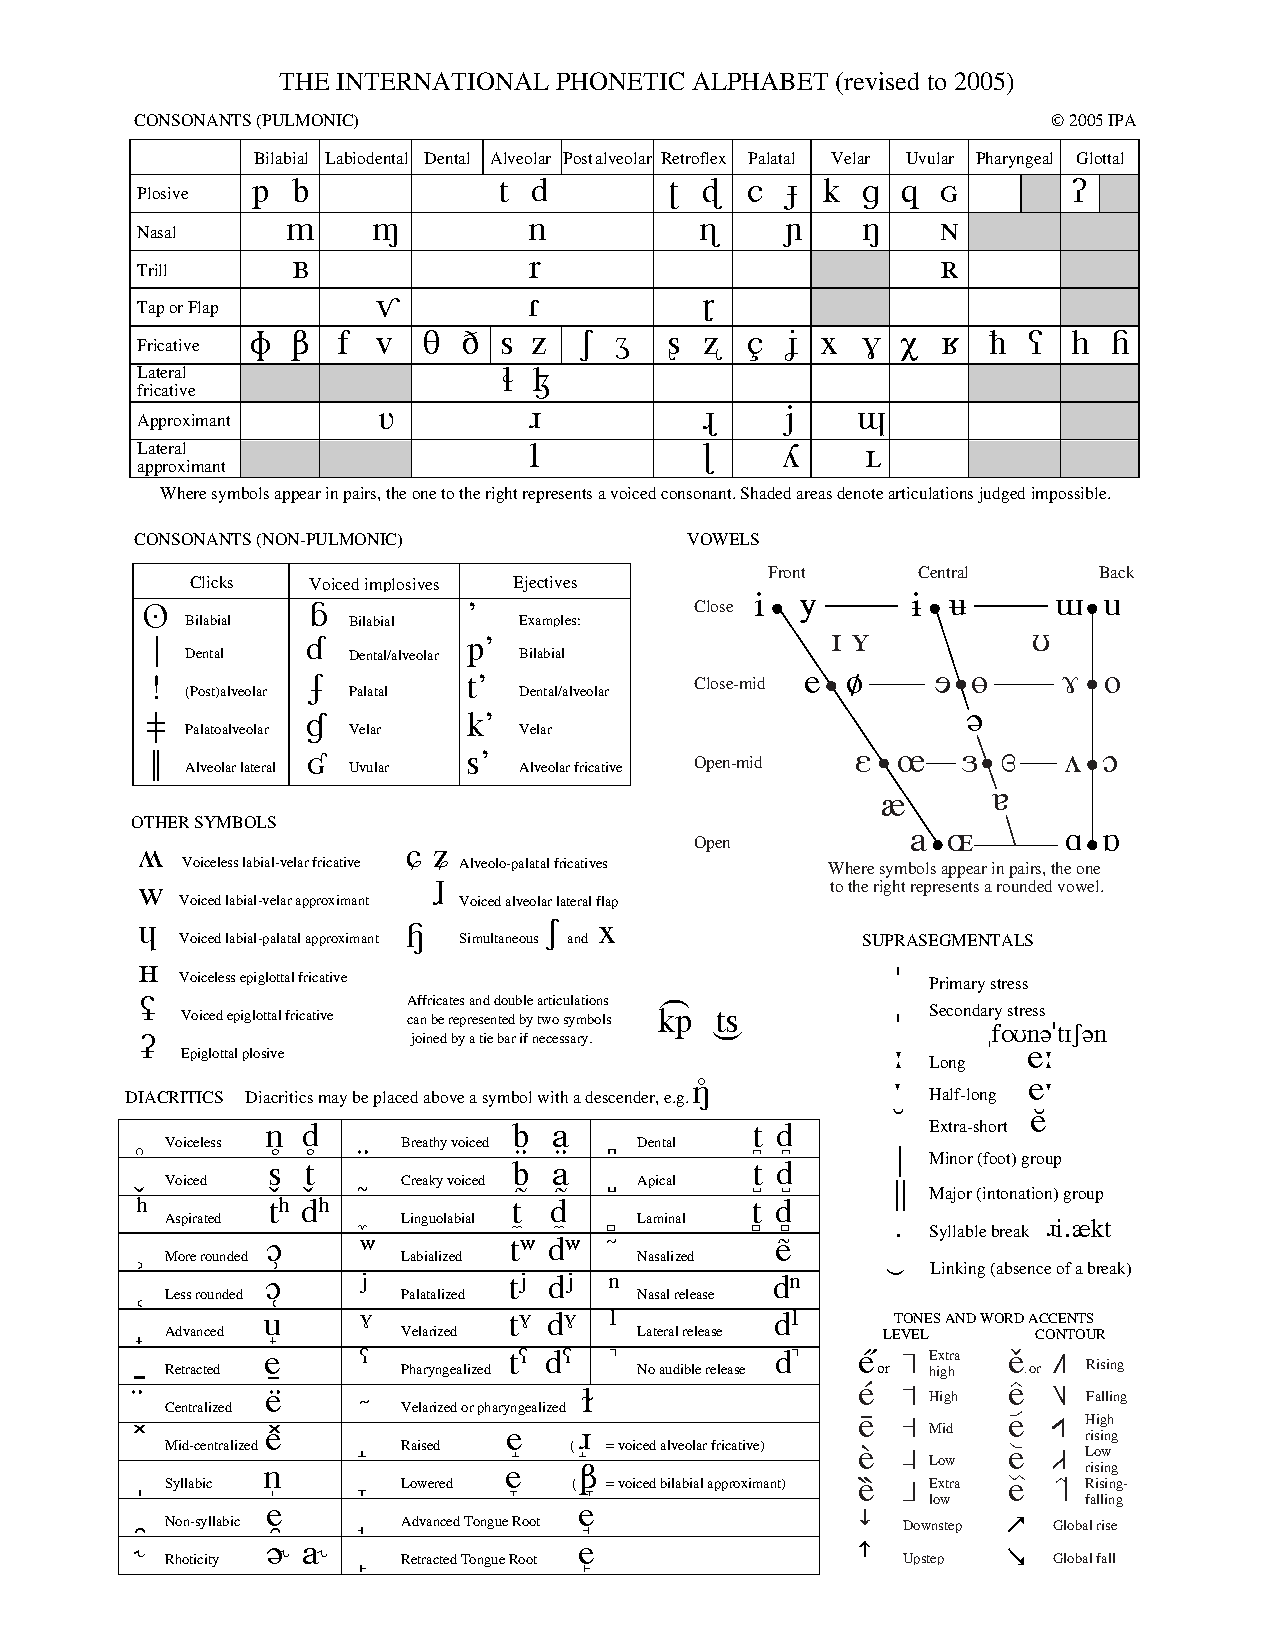
\includegraphics[width=0.7\paperwidth]{gfx/ipa-chart-2005.pdf}}
        \caption{IPA Chart.}\label{fig:ipa-chart}
\end{figure}


The phones in the \ac{IPA} chart are organised into tables which take into account several properties of the sounds, such as major classes (e.g. ``pulmonic consonants'' or ``vowels''); manner of articulation (e.g. ``plosive'', ``nasal'' or ``trill''); place of articulation (e.g. ``bilabial'', ``dental'' or ``alveolar''); status of the glottis (e.g. ``voiced'', ``voiceless'' or ``aspirated''); type of stress (e.g. ``primary'' or ``secondary''); as well as some other segmental or supra-segmental aspects. For English and \gls{BP}, the most relevant tables are the ones which contain pulmonic consonants, the table at the top, and vowels, the diagram in the centre-right position. These two tables indicate the two major classes of sound, the term refers to the main types of sound produced by the open vs closed possibilities of vocal tract variation \cite{Crystal2011}.

Pulmonic consonants are organised as follows: rows designate the manner of articulation, i.e. how the consonant is produced; and columns describe the place of articulation, i.e. where in the phonatory system tract the consonant is articulated. Each cell in the table may contain up to two phones, those which are aligned to the left are voiceless (meaning that the glottis is open when they are produced); and those which are aligned to the right are voiced (which means that the glottis is closed when the phone is uttered). 

One refers to each phone by describing its phonetic properties, for instance, the first phone in the table is [\ipa{p}], a voiceless bilabial plosive. It means that the symbol [\ipa{p}] corresponds to a consonant which is produced with a movement of both lips, with the glottis open, in a plosive manner. In other words, [\ipa{p}] describes the sound that is made by first blocking the airflow with both lips closed so that no air can pass, and then by increasing the pressure inside the vocal tract in such a way that the air pressure is so high that it bursts the region where it was blocked and passes through the lips, producing sound.

The voiced counterpart of [\ipa{p}] is [\ipa{b}], a voiced bilabial plosive, which means that [\ipa{b}] is produced in the same way of [\ipa{p}], except that for [\ipa{b}], the glottis is closed and not open when the air bursts through the lips. To give a few more examples of how symbols are referred to: [\ipa{n}] is called an alveolar nasal, [\ipa{S}] is a voiceless postalveolar fricative, [\ipa{H}] is a voiced glotal fricative and so on.

Vowels, on the other hand, are described with a different set of properties. The vowel diagram (also called vowel trapezium) provides a schematic arrangement of the vowels which summarises the vowel height of the tongue and/or jaw, as well as how far back the tongue is for articulating each vowel. The vertical position indicates the vowel height, which is related to how close the tongue is to the roof of the mouth or how open is the jaw. Close vowels, which are produced with the tongue close to the roof of the mouth, such as the segment [\ipa{u}] in \pt{\textbf{u}va} (grape), are placed at the top of the diagram. In contrast, open vowels, i.e. those which are pronounced with the jaw open or with the tongue distant from the roof of the mouth, such as the [\ipa{a}] in \pt{\textbf{a}ve} (bird), are at the bottom of the vowel trapezium. The horizontal position reveals the vowel backness, or the place of the tongue relative to the back of the mouth. Front vowels, such as [\ipa{i}] as in \pt{p\textbf{i}pa} (kite), are found in the left part of the vowel diagram; whereas back vowels, like [\ipa{O}] in \pt{r\textbf{o}\c{c}a} (small farm), are on the right side.

Vowels and consonants are put together in sequence in order to form syllables, words, phrases and sentences. As in Portuguese we use a script that is quite transparent in terms of letter-to-sound conversion, we tend to assume a one-to-one relation between the number of letters in a word and the number of phones it contains, but this is not always true. For instance, the word \pt{t\'axi} (taxi) has four letters, but five phones: [\ipa{"tak.sI}]; in contrast, \pt{aqui} (here) has four letters but only three phones [\ipa{a"ki}]. Despite their close relation, one must not mistaken letters for phone symbols, the former refers to written language and the latter to the speech stream.

With respect to Phonology, it is considered the branch of linguistics which studies the sound systems of languages \cite{Crystal2011}. Phonology is concerned with describing the sound inventories of languages, focusing on sounds which are used distinctively, i.e. those which are capable of distinguishing the meaning of two words. For instance, in English, the words \eng{tip} [\ipa{"tIp}] and \eng{chip} [\ipa{"tSIp}] have different meaning: the former is a sum of money that is given to someone as a reward or payment for a service; whereas the latter is a hardware component. In terms of phonetics, these words are only different with respect to their initial phone, \eng{tip} is produced with an alveolar plosive [\ipa{t}], whereas \eng{chip} begins with an alveopalatal plosive [\ipa{tS}]. This shows that [\ipa{t}] and [\ipa{tS}] can be used distinctively in English, therefore, they are considered phonemes of English. Traditionally, phones are represented inside slashes, thus /t/ and /tS/.

On the other hand, in Portuguese, if one says \pt{tia} (aunt) with an alveolar plosive [\ipa{t}] or an alveopalatal [\ipa{tS}], the meaning of the word does not change, both [\ipa{"ti6}] and [\ipa{"tSi6}] refer to the same kinship relation in Portuguese: the sister of one's parents or the wife of one's uncle. The phones [\ipa{t}] and [\ipa{tS}], in this context, do not change the meaning, i.e. they are not distinctive; due to this, they are not considered phonemes, but allophones of a single phoneme /t/. Phonemes are abstract units, allophones and phones, on the other hand, are concrete, they are part of realization.

Summarising, Phonology will analyse speech from the perspective of sound patterns and sound structure. Phonology studies speech from the perspective of abstract units, called phonemes, which have the core property of being able to distinguish the meaning of words, i.e. to be used distinctively. By convention, phonemes are represented inside slashes, often using symbols from the \ac{IPA} (but not always).

\subsection{The Phonetic Inventory of Brazilian Portuguese} 

There is much debate about which set of phones best describes the phonetic inventory of \gls{BP}. Several analyses have been proposed by different researchers through the years \cite{Bisol2005, Cagliari2002, Camara1970, Cristofaro2005, Neves1999}, and despite the fact that the analyses usually concur with respect to core questions, there is a lot of disagreement in terms of convention and the usage of different phones.  For instance, some authors propose that the postonic ``a'' should be transcribed as [\ipa{5}], whereas others argue that it is more centralized and closer to the schwa [\ipa{@}]. Similarly, some researchers defend that the glides in Portuguese have a stronger consonantal aspect, thus being transcribed [\ipa{w}] and [\ipa{j}]; at the same time, others argue for a more vocalic nature of these sounds and prefer to represent them as [\ipa{\textsubarch{U}}] and [\ipa{\textsubarch{I}}] respectively. 

For the sake of this thesis, we will presented a simplified version of the analysis put forward by \citet{Cristofaro2005}. The work of \citet{Cristofaro2005} is widely known and well-established in the area of Phonetics and Phonology for \ac{BP}; we use it as a reference and present here a simplified version of the analysis, assuming a standard dialect and less linguistic variability, which we find more suitable for Natural Language Processing systems.

The phonetic inventory of \ac{BP} can be defined using 43 phones for describing (26 consonants and 17 vowels), all segments are grouped into \autoref{tab:pt-br-consonants}, \autoref{fig:pt-br-vowels} and \autoref{fig:pt-br-nasal-vowels}.

{\renewcommand{\arraystretch}{0.8}
\begin{table}[!ht]
\centering
\setlength{\tabcolsep}{0.4em}
\caption{Brazilian Portuguese consonants.}
\begin{tabular}{|l|lr|lr|lr|lr|lr|lr|lr|}
\hline
 & \multicolumn{ 2}{c|}{\scriptsize Bilabial} & \multicolumn{ 2}{c|}{\scriptsize Labiod.} & \multicolumn{ 2}{c|}{\scriptsize Alveolar} & \multicolumn{ 2}{c|}{\specialcell[t]{\scriptsize Postalv.}} & \multicolumn{ 2}{c|}{\scriptsize Palatal} & \multicolumn{ 2}{c|}{\scriptsize Velar} & \multicolumn{ 2}{c|}{\scriptsize Glottal} \\ \hline
\scriptsize Plosive & \ipa{p} & \ipa{b} &  &  & \ipa{t} & \ipa{d} &  &  &  &  & \ipa{k} & \ipa{g} &  &  \\ \hline
\scriptsize Affricate &  &  &  &  & \ipa{tS} & \ipa{dZ} &  &  &  &  &  &  &  &  \\ \hline
\scriptsize Nasal &  & \ipa{m} &  &  &  & \ipa{n} &  &  &  & \ipa{\textltailn} &  &  &  &  \\ \hline
\scriptsize Trill &  &  &  &  &  & \ipa{r} &  &  &  &  &  &  &  &  \\ \hline
\specialcell[t]{\scriptsize Tap} &  &  &  &  &  & \ipa{R} &  &  &  &  &  &  &  &  \\ \hline
\scriptsize Fricative &  &  & \ipa{f} & \ipa{v} & \ipa{s} & \ipa{z} & \ipa{S} & \ipa{Z} &  &  & \ipa{x} & \ipa{G} & \ipa{h} & \ipa{H} \\ \hline
\scriptsize Approximant &  &  &  &  &  & \ipa{\*r}  &  &  &  & \ipa{j} &  & \ipa{w} &  &  \\ \hline
\scriptsize Lateral Appr.  &  &  &  &  &  & \ipa{l} &  &  &  & \ipa{L} &  &  &  &  \\ \hline
\end{tabular}
\label{tab:pt-br-consonants}
\end{table}
\renewcommand{\arraystretch}{1}}

{\begin{figure}[!ht]
\caption{Brazilian Portuguese oral vowels.}
\centering
\begin{vowel}
    \putcvowel[l]{\ipa{i}}{1}
    \putcvowel[l]{\ipa{e}}{2}
    \putcvowel[l]{\ipa{E}}{3}
    \putcvowel[l]{\ipa{a}}{4}
    \putcvowel{\ipa{I}}{13}
    \putcvowel[r]{\ipa{O}}{6}
    \putcvowel[r]{\ipa{o}}{7}
    \putcvowel[r]{\ipa{u}}{8}
    \putcvowel{\ipa{@}}{11}
    \putcvowel{\ipa{U}}{14}
\end{vowel}
\label{fig:pt-br-vowels}
\end{figure}}

{\begin{figure}[!ht]
\caption{Brazilian Portuguese nasal vowels.}
\centering
\begin{vowel}
    \putcvowel[l]{\ipa{\~i}}{1}
    \putcvowel[l]{\ipa{\~e}}{2}
    \putcvowel[l]{\ipa{\~a}}{15}
    \putcvowel{\ipa{\~I}}{13}
    \putcvowel[r]{\ipa{\~o}}{7}
    \putcvowel[r]{\ipa{\~u}}{8}
    \putcvowel{\ipa{\~U}}{14}
\end{vowel}
\label{fig:pt-br-nasal-vowels}
\end{figure}}

As one might notice from \autoref{tab:pt-br-consonants}, there are six plosive consonants in 
\gls{BP}, namely [\ipa{p, b, t, d, k, g}]. As previously said, plosive sounds are produced by first blocking the airflow so that no air can pass the vocal tract, and then by increasing the pressure in such a way that the bursts through the vocal tract, creating sound. Plosive sounds are also called ``stops'' or ``occlusives''. In \ac{BP} plosive sounds usually occupy the onset position of a syllabe (i.e. the initial position) as the [\ipa{p}] in \pt{\textbf{p}ato} (duck). Some other examples can be found in \autoref{tab:pt-br-plosive-i}:

\begin{table}[!ht]
\caption{Examples of plosive consonants in Brazilian Portuguese (First table).}
\centering
\small
\begin{tabular}{ccccc}
\hline
Phone & Transcription & Word & Translation & Description \\ \hline
\normalsize [\ipa{p}] & [\ipa{p}]ato & pato & duck & voiceless bilabial plosive \\
\normalsize [\ipa{b}] & [\ipa{b}]ato & bato & (I) hit & voiced bilabial plosive \\
\normalsize [\ipa{t}] & mo[\ipa{t}]o & moto & bike & voiceless alveolar plosive \\
\normalsize [\ipa{d}] & mo[\ipa{d}]o & modo & way & voiced alveolar plosive \\
\normalsize [\ipa{k}] & [\ipa{k}]ato & cato & duck & voiceless velar plosive \\
\normalsize [\ipa{g}] & [\ipa{g}]ato & gato & cat & voiced velar plosive \\ \hline
\end{tabular}
\label{tab:pt-br-plosive-i}
\end{table}

Plosives in \gls{BP} might also occur in postvocalic position (i.e. the end of a syllable), for instance, as in the [\ipa{p}] \pt{a[\ipa{p.}]to} (able.MASC.SG). However, when plosives occupy postvocalic position in \ac{BP}, a phonological process called epenthesis will often take place, giving rise to a new syllable structure: a[\ipa{.pI.}]to \cite{Collischonn2004}. Epenthesis is phonological process in which an extra sound is inserted in the word, also known as intrusion. A few other examples are shown in \autoref{tab:pt-br-plosive-ii}:

\begin{table}[!ht]
\caption{Examples of plosive consonants in Brazilian Portuguese (Second table).}
\centering
\small
\begin{tabular}{ccccc}
\hline
Phone & Transcription & Word & Translation & Description \\ \hline
\normalsize [\ipa{p}] & [\ipa{ap.}]$\sim$[\ipa{a.pI.}]to & apto & able.MASC.SG & voiceless bilabial plosive \\
\normalsize [\ipa{b}] & [\ipa{ab.}]$\sim$[\ipa{a.bi.}]dicar & abdicar & to abdicate & voiced bilabial plosive \\
\normalsize [\ipa{t}] & [\ipa{at.}]$\sim$[\ipa{a.ti.}]$\sim$[\ipa{a.tSi.}]mosfera & atmosfera & atmosphere & voiceless alveolar plosive \\
\normalsize [\ipa{d}] & [\ipa{ad.}]$\sim$[\ipa{a.di.}]$\sim$[\ipa{a.dZi.}]ministrar & administrar & to manage & voiced alveolar plosive \\
\normalsize [\ipa{k}] & [\ipa{fik.}]$\sim$[\ipa{fi.ki.}]\c{c}\~ao & fic\c{c}\~ao & fiction & voiceless velar plosive \\
\normalsize [\ipa{g}] & [\ipa{dOg.}]$\sim$[\ipa{dO.gI.}]ma & dogma & dogma & voiced velar plosive \\ \hline
\end{tabular}
\label{tab:pt-br-plosive-ii}
\end{table}

\ac{BP} also has two affricate sounds, both are produced in the postalveolar region: [\ipa{tS}] and [\ipa{dZ}]. Affricate sounds are those that begin by completely stopping the airflow then suddenly releasing it in a constricted way. In other words, affricates begin with a stop and then are released with a fricative sound, e.g. [\ipa{tS}] has two stages, it starts with a [t] stop and then the air is set free with a fricative sound [\ipa{S}]. 

Affricate phones are often positional variants of [\ipa{t}] and [\ipa{d}], when these are followed by the high vowels [\ipa{i, I, \~i}], or when they occupy postvocalic position. For example, in several dialects of \gls{BP}, the word \pt{tia} (aunt) is realised as [\ipa{"tSi@}] with an initial voiceless postalveolar affricate [\ipa{tS}]. Similarly, \pt{dia} (day) is often pronounced as [\ipa{"dZi@}]. This phenomenon is called palatalisation and it results from an overlap among the speech gestures for [\ipa{t, d}] and high vowels [\ipa{i, I, \~i}]; basically these consonants change their place and manner of articulation in order to anticipate the gestures which are necessary for producing those high vowels. 

When [\ipa{t}] and [\ipa{d}] are produced as [\ipa{tS}] and [\ipa{dZ}] due to the presence of a high vowel, they are called positional variants or allophones. Even though in \ac{BP}, [\ipa{tS}] and [\ipa{dZ}] are mainly allophones, there are a few cases when they are not, as the ``tch'' in \pt{\textbf{tch}u\textbf{tch}uca} (slang:pussycat) or the ``dj'' in \pt{\textbf{Dj}avan} (a personal name). It is worth pointing out that in a few dialects of \ac{BP}, palatalisation is a much broader phenomenon which affects other contexts as well \cite{Cristofaro2012}. A few other examples of words with affricates are provided in \autoref{tab:pt-br-affricates}.

\begin{table}[!ht]
\caption{Examples of affricate consonants in Brazilian Portuguese.}
\centering
\small
\begin{tabular}{ccccc}
\hline
Phone & Transcription & Word & Translation & Description \\ \hline
\normalsize [\ipa{tS}] & [\ipa{tSi}]a & tia & aunt & voiceless postalveolar affricate \\
\normalsize [\ipa{tS}] & [\ipa{atS.}]mosfera & atmosfera & atmosphere & voiceless postalveolar affricate \\
\normalsize [\ipa{tS}] & [\ipa{tS}]u[\ipa{tS}]uca & tchutchuca & pussycat & voiceless postalveolar affricate \\
\normalsize [\ipa{dZ}] & [\ipa{dZi}]a & dia & day & voiced postalveolar affricate \\
\normalsize [\ipa{dZ}] & [\ipa{adZ.}]ministrar & administrar & to manage & voiced postalveolar affricate \\
\normalsize [\ipa{dZ}] & [\ipa{dZ}]avan & Djavan & personal name & voiced postalveolar affricate \\ \hline
\end{tabular}
\label{tab:pt-br-affricates}
\end{table}

There are three nasal consonants in \ac{BP}, viz. [\ipa{m, n, \textltailn}]. Nasal consonants are produced with the velum lowered, in a way that the air is free to pass through the nose. In current language usage, due to vowel nasalisation, nasal consonants in \ac{BP} are basically limited to syllable initial position, for example, as the ``m'' in \pt{\textbf{m}ar} (sea), the ``n'' in \pt{\textbf{n}\~ao} (no) or the ``nh'' in \pt{rai\textbf{nh}a} (queen) respectively. It is important to notice that in words such as \pt{ambos} (both) or \pt{anta} (tapir), nasalisation most of the time will take place. It means that the gesture for lowering the velum will happen during the articulation of the vowel, in such a way that the vowel will be entirely nasalized and the nasal consonant will not perceived as a segment \cite{Medeiros2007}, i.e. \pt{ambos} will be produced as [\ipa{"\~a.bUs}] and \pt{anta} will become [\ipa{"\~a.t@}] with no explicit nasal consonant. A few examples of \ac{BP} words with nasal consonants can be found in \autoref{tab:pt-br-nasal-cons}, we also provide some counter-examples of vowel nasalisation.

\begin{table}[!ht]
\caption{Examples of nasal consonants and nasal vowels in Brazilian Portuguese.}
\centering
\small
\begin{tabular}{ccccc}
\hline
Phone & Transcription & Word & Translation & Description \\ \hline
\normalsize [\ipa{m}] & ca[m]a & cama & bed & bilabial nasal \\
\normalsize [\ipa{n}] & ca[n]a & cana & sugar cane & alveolar nasal \\
\normalsize [\ipa{\textltailn}] & ba[\ipa{\textltailn}]a & banha & fat & palatal nasal \\
\normalsize [\ipa{\~a}] & [\ipa{\~a}]t\^onio & Ant\^onio & personal name & nasal [\ipa{\~a}] \\
\normalsize [\ipa{\~e}] & l[\ipa{\~e}]brar & lembrar & remember & nasal [\ipa{\~e}] \\
\normalsize [\ipa{\~i}] & [\ipa{\~i}]teresse & interesse & interest & nasal [\ipa{\~i}] \\
\normalsize [\ipa{\~o}] & [\ipa{\~o}]bro & ombro & shoulder & nasal [\ipa{\~o}] \\
\normalsize [\ipa{\~u}] & [\ipa{\~u}]tar & untar & grease & nasal [\ipa{\~u}] \\ \hline
\end{tabular}
\label{tab:pt-br-nasal-cons}
\end{table}

The sounds [\ipa{r, R, \*r, x, G, h, H}] are called rhotics because they represent sounds which are somehow related to the letter ``r'' -- ``rho'' in Greek. Although some of these sounds are quite different in terms of phonetics, they have shown to behave similarly with respect to phonology in many languages \cite{Wiese2001}.

The first one, called alveolar trill [\ipa{r}] is found in some dialects of \ac{BP} -- especially in southern Brazil -- and is also known as rolled-r. The alveolar trill is produced by making the tip of the tongue touch the alveolar ridge repeatedly, interrupting the airflow. This sound is part of the rhotic class (i.e. the r-like) and for the dialects which have it, it corresponds, for instance, to the ``r'' in \pt{carta} (letter) or the ``rr'' in \pt{carro} (car). The trill [\ipa{r}] is closely related to the alveolar tap [\ipa{R}], the only difference being that the tap touches the gum ridge once, whereas the trill does it several times. This distinction is found in Spanish, e.g. in \pt{perro} [\ipa{pE.ro}] vs. \pt{pero} [\ipa{pE.Ro}]. 

In terms of articulatory gesture, the trill [\ipa{r}] resembles the alveolar tap [\ipa{R}], the difference is that the tap touches the gum ridge once, whereas the trill does it several times. Both these phones are used distinctively in languages such as Spanish, e.g. in \pt{perro} [\ipa{pE.ro}] vs. \pt{pero} [\ipa{pE.Ro}]. In Portuguese, the tap [\ipa{R}] can be found in all dialects, the thrill [\ipa{r}], on the other hand, is limited to regional dialects. It occurs basically in two contexts, between two vowels, e.g. \pt{arara} (parrot), or in complex onsets, such as ``br'' in \pt{cabrita} (female goat).

The alveolar approximant [\ipa{\*r}] is the sound which corresponds to the so-called ``r-caipira'' in \ac{BP}. It is an approximant consonant, which means that the vocal tract is narrowed, but the level of constriction is not sufficient to generate hiss or turbulence. In the dialects in which this rhotic sound occur, it is found mostly at the end of a syllable, as the ``r'' in \pt{amor} (love) or \pt{porta} (door)

The other rhotics variants [\ipa{x, G, h, H}] can be considered free variants or free allophones among themselves, they are also referred to as strong-r, in contrast with the tap. The first two, [\ipa{x, G}] are velar fricative sounds consonants, in other words, they are produced in such a way that the airflow passes through the vocal tract with constriction and turbulence and their place of articulation is near the soft palate. The phone [\ipa{x}] corresponds to a voiceless sound, which means that the air passes freely through the vocal folds, i.e. they are open. On the other hand, [\ipa{G}] is a voiced velar fricative, which means that it puts the vocal folds to vibrate when it is produced. The phones [\ipa{h, H}] are articulated in the region of the glottis and they also show constriction in the air passage, that is why the are called glottal fricatives. Analogously to [\ipa{x, G}], [\ipa{h, H}] also present the voiceless-voiced dichotomy; the vocal folds are open when [\ipa{h}] is produced, but they are closed and vibrate in [\ipa{H}]. \autoref{tab:pt-br-rhotics} presents some examples of words with rhotic sounds in \ac{BP}.

\begin{table}[!ht]
\caption{Examples of rhotics in Brazilian Portuguese.}
\centering
\small
\begin{tabular}{ccccc}
\hline
Phone & Transcription & Word & Translation & Description \\ \hline
\normalsize [\ipa{r, x, G, h, H}] & [\ipa{r, x, G, h, H}]ato & rato & mouse & strong-r \\
\normalsize [\ipa{r, x, G, h, H}] & [\ipa{r, x, G, h, H}]oma & Roma & Rome & strong-r \\
\normalsize [\ipa{r, x, G, h, H}] & mo[\ipa{r, x, G, h, H}]o & morro & hill & strong-r \\
\normalsize [\ipa{r, x, G, h, H}] & mo[\ipa{r, x, G, h, H}]o & carro & car & strong-r \\
\normalsize [\ipa{r, \*r, x, G, h, H}] & amo[\ipa{r, \*r, x, G, h, H}] & amor & love & strong-r \\
\normalsize [\ipa{r, \*r, x, G, h, H}] & dan\c{c}a[\ipa{r, \*r, x, G, h, H}] & dan\c{c}ar & to dance & strong-r \\
\normalsize [\ipa{r, \*r, x, h}] & mo[\ipa{r, \*r, x, h}]to & morto & dead & strong-r \\
\normalsize [\ipa{r, \*r, x, h}] & po[\ipa{r, \*r, x, h}]co & porco & pig & strong-r \\
\normalsize [\ipa{r, \*r, G, H}] & mo[\ipa{r, \*r, G, H}]da & morda & bite & strong-r \\
\normalsize [\ipa{r, \*r, G, H}] & ca[\ipa{r, \*r, G, H}]ga & carga & load & strong-r \\
\normalsize [\ipa{R}] & ca[\ipa{R}]o & caro & expensive.MASC.SG & alveolar tap \\
\normalsize [\ipa{R}] & i[\ipa{R}]a & ira & wrath & alveolar tap \\
\normalsize [\ipa{R}] & a[\ipa{R}]a[\ipa{R}]a[\ipa{R}]qua[\ipa{R}]a & Araraquara & city name & alveolar tap \\
\normalsize [\ipa{R}] & a[\ipa{.bR}]ir & abrir & to open & alveolar tap \\
\normalsize [\ipa{R}] & co[\ipa{.bR}]a & cobra & snake & alveolar tap \\ \hline
\end{tabular}
\label{tab:pt-br-rhotics}
\end{table}

Apart from the rhotic ones, \ac{BP} has six more fricative sounds: [\ipa{f, v, s, z, S, Z}]. The first two are named labiodental because they are produced by making the lips touch the upper teeth. As other fricative sounds, the air for [\ipa{f, v}] does not passes freely in the vocal tract, on contrary it finds obstacles thus generating turbulence. With respect to [\ipa{s, z}], both are articulated in the region of the alveolar ridge, that is why they are called alveolar fricatives. Finally, [\ipa{S, Z}] are produced more towards the back of the vocal tract, in a place between the alveolar ridge and the hard palate; this is the reason why they are referred to as postalveolar or palato-alveolar consonants. All these six fricative sounds can be found in all dialects of \ac{BP} in onset position, as can be seen from the examples in \autoref{tab:pt-br-fricatives-onset}.

\begin{table}[!ht]
\caption{Examples of fricative consonants in Brazilian Portuguese (onset).}
\centering
\small
\begin{tabular}{ccccc}
\hline
Phone & Transcription & Word & Translation & Description \\ \hline
\normalsize [\ipa{f}] & [\ipa{f}]aca & faca & knife & voiceless bilabial plosive \\
\normalsize [\ipa{v}] & [\ipa{v}]aca & vaca & cow & voiced bilabial plosive \\
\normalsize [\ipa{s}] & ca[\ipa{s}]a & ca\c{c}a & hunt & voiceless alveolar plosive \\
\normalsize [\ipa{z}] & ca[\ipa{z}]a & casa & house & voiced alveolar plosive \\
\normalsize [\ipa{S}] & quei[\ipa{S}]o & queixo & chin & voiceless bilabial plosive \\
\normalsize [\ipa{Z}] & quei[\ipa{Z}]o & queijo & cheese & voiceless bilabial plosive \\ \hline
\end{tabular}
\label{tab:pt-br-fricatives-onset}
\end{table}

In postvocalic position, [\ipa{f, v, s, z, S, Z}] show a different behaviour. The labiodental fricatives [\ipa{f, v}] act similarly to the plosives summarised in \autoref{tab:pt-br-plosive-ii}, they may occupy the final position of a syllable, e.g. a[\ipa{f}]ta (cold sore), but epenthesis will often take place: a[\ipa{.fI.}]ta. Alveolar fricatives are present in postvocalic position in most dialects of \ac{BP}. Some regions of Brazil have postalveolar fricatives [\ipa{S, Z}] instead, notably the dialect spoken in Rio de Janeiro. For [\ipa{s, z, S, Z}], anticipatory assimilation more often than not will occur, thus the choice between [\ipa{s, S}] and [\ipa{z, Z}] will depend on the following consonant, if it is voiced, then the fricative will also be voiced. For example, the fricative in \pt{rasgar} (to rip) is voiced: ra[\ipa{z}]gar; but the one in \pt{costa} (coast) is not: co[\ipa{s}]ta. The same distinction will be present in dialects with the postalveolar fricatives [\ipa{S, Z}]. In \autoref{tab:pt-br-fricatives-coda}, one can find more examples of fricatives in postvocalic position in \ac{BP}.

\begin{table}[!ht]
\caption{Examples of fricative consonants in Brazilian Portuguese (postvocalic).}
\centering
\small
\begin{tabular}{ccccc}
\hline
Phone & Transcription & Word & Translation & Description \\ \hline
\normalsize [\ipa{f}] & [\ipa{af.}]$\sim$[\ipa{a.fI.}]ta & apto & able.MASC.SG & voiceless bilabial plosive \\
\normalsize [\ipa{f}] & [\ipa{of.}]$\sim$[\ipa{o.fi.}]talmologia & oftalmologia & ophthalmology & voiceless bilabial plosive \\
\normalsize [\ipa{s}] & po[\ipa{s, S}]tar & postar & to post & voiceless bilabial plosive \\
\normalsize [\ipa{s}] & ca[\ipa{s, S}]tor & castor & beaver & voiced bilabial plosive \\
\normalsize [\ipa{z}] & de[\ipa{z, Z}]gaste & desgaste & wear and tear & voiceless alveolar plosive \\
\normalsize [\ipa{z}] & tran[\ipa{z, Z}]gressivo & transgressivo & transgressive.MASC.SG & voiced alveolar plosive \\ \hline
\end{tabular}
\label{tab:pt-br-fricatives-coda}
\end{table}

Glides (also known as semivowels) are phones which are similar to vowels in terms of acoustics or articulation, but which function as consonants in terms of phonotactics, in other words, they are not placed in the nucleus of a syllable. There are two glides in \ac{BP}, one which has its place of articulation in the velar region [\ipa{w}] and another one which is produced near the hard palate [\ipa{j}]. Acoustically, the velar glide [\ipa{w}] is very similar to the vowel [\ipa{U}], and palatal glide is very close to [\ipa{I}]. The debate whether these sounds should be considered vowels or glides is beyond the scope of this thesis. \autoref{tab:pt-br-glides} presents some examples with glides.

\begin{table}[!ht]
\caption{Examples of glides in Brazilian Portuguese.}
\centering
\small
\begin{tabular}{ccccc}
\hline
Phone & Transcription & Word & Translation & Description \\ \hline
\normalsize [\ipa{w}] & c\'e[\ipa{w}] & c\'eu & sky & voiceless bilabial plosive \\
\normalsize [\ipa{w}] & pa[\ipa{w}] & pau & stick & voiceless bilabial plosive \\
\normalsize [\ipa{w}] & cinq[\ipa{w}]enta & cinquenta & fifty & voiceless bilabial plosive \\
\normalsize [\ipa{j}] & fu[\ipa{j}] & fui & (I) was & voiceless bilabial plosive \\
\normalsize [\ipa{j}] & pa[\ipa{j}]x\~ao & paix\~ao & passion & voiceless bilabial plosive \\
\normalsize [\ipa{j}] & ce[\ipa{j}]a & ceia & supper & voiceless bilabial plosive \\ \hline
\end{tabular}
\label{tab:pt-br-glides}
\end{table}

\ac{BP} has two consonants which are articulated by making the air escape the vocal tract around the sides of the tongue: [\ipa{l, L}]; due to this articulatory aspect, these sounds are called lateral consonants. The former [\ipa{l}] is named lateral alveolar since it is produced in the region of the gum ridge. The latter is articulated with the body of the tongue reaching the hard palate, thus [\ipa{L}] is considered a lateral palatal consonant. In terms of context of occurrence, both laterals show a very different distribution.

The alveolar lateral is present in onset position in all dialects of \ac{BP}. It corresponds to the ``l'' in words like \pt{lata} (can) or \pt{pular} (to skip). However, in postvocalic position, [\ipa{l}] commonly undergoes vocalisation, and is produced as a vowel [\ipa{\textsubarch{U}}] or glide [\ipa{w}], for example, in \pt{sal} (salt) or \pt{Sol} (sun), both ``l'' are frequently pronounced as vowels or glides, instead of consonant. 

As for the palatal lateral, it is limited to syllable initial position and generally corresponds to the letters ``lh'' in writing, e.g. \pt{lhama} (llama) or \pt{alho} (garlic). A few other examples of words with laterals can be seen in \autoref{tab:pt-br-laterals}.

\begin{table}[!ht]
\caption{Examples of lateral consonants in Brazilian Portuguese.}
\centering
\small
\begin{tabular}{ccccc}
\hline
Phone & Transcription & Word & Translation & Description \\ \hline
\normalsize [\ipa{l}] & sa[\ipa{l}]a & sala & classroom & voiceless bilabial plosive \\
\normalsize [\ipa{l}] & [\ipa{l}]an\c{c}a & lan\c{c}a & spear & voiced bilabial plosive \\
\normalsize (l-vocalisation) & sa[\ipa{w}]to & salto & jump & voiceless alveolar plosive \\
\normalsize (l-vocalisation) & ca[\ipa{w}]da & calda & syrup & voiced alveolar plosive \\
\normalsize [\ipa{L}] & a[\ipa{L}]eio & alheio & someone else's & voiceless bilabial plosive \\
\normalsize [\ipa{L}] & o[\ipa{L}]ar & olhar & look & voiceless bilabial plosive \\ \hline
\end{tabular}
\label{tab:pt-br-laterals}
\end{table}

With respect to vowels, as it can be observed in \autoref{fig:pt-br-vowels}, \ac{BP} has ten oral vowels: [\ipa{i, I, e, E, a, @, O, o, u, U}]. Different from consonants, vowels are described in terms of height, backness and roundedness. Height refers how close the tongue is to the roof of the mouth or how open the jaw is. Backness describes how retracted the tongue is relative to the back of the mouth. Finally roundedness indicates the position of the lips when the vowel is articulated.

\ac{BP} has four vowels which are produced forward in the mouth [\ipa{i, I, e, E, a}], all of which are not rounded. There are four back vowels [\ipa{O, o, u, U}], which are all rounded, i.e. they are produced with lip protrusion. One central vowel [\ipa{@}] -- also called ``schwa'' -- also exists in \ac{BP}.

The vowels [\ipa{i, e, E, a, O, o, u}] are considered tense, which means that they occur in pretonic or tonic syllables; whereas [\ipa{I, @, U}] are relaxed, being found just in postonic contexts. A few examples of vowels in \ac{BP} can be seen in \autoref{tab:pt-br-vowels-examples} and \autoref{tab:pt-br-vowels-examples-post}. As one might see from the examples, the distribution of vowels in \ac{BP} is deeply influenced by the lexical stress, postonic syllables use just a subset of the vowels which are present in pretonic or tonic syllables.

\begin{table}[!ht]
\caption{Examples of vowels in Brazilian Portuguese (pretonic and tonic).}
\centering
\small
\begin{tabular}{ccccc}
\hline
Phone & Transcription & Word & Translation & Description \\ \hline
\normalsize [\ipa{i}] & S[\ipa{i}]b\'eria & Sib\'eria & Siberia & high front unrounded vowel \\
\normalsize [\ipa{i}] & b[\ipa{i}]co & bico & nib & high front unrounded vowel \\
\normalsize [\ipa{i}] & s[\ipa{i}]go & sigo & (I) follow & high front unrounded vowel \\

\normalsize [\ipa{e}] & p[\ipa{e}]dalar & pedalar & to pedal & mid-high front unrounded vowel \\
\normalsize [\ipa{e}] & p[\ipa{e}]ra & pera & pear & mid-high front unrounded vowel \\
\normalsize [\ipa{e}] & p[\ipa{e}]sames & p\^esames & condolence & mid-high front unrounded vowel \\

\normalsize [\ipa{E}] & p[\ipa{E}]zinho & pezinho & little foot & mid-low front unrounded vowel \\
\normalsize [\ipa{E}] & p[\ipa{E}]ste & peste & plague & mid-low front unrounded vowel \\
\normalsize [\ipa{E}] & p[\ipa{E}] & p\'e & foot & mid-low front unrounded vowel \\

\normalsize [\ipa{a}] & g[\ipa{a}]linha & galinha & chicken & low front unrounded vowel \\
\normalsize [\ipa{a}] & c[\ipa{a}]sa & casa & house & low front unrounded vowel \\
\normalsize [\ipa{a}] & ch[\ipa{a}] & ch\'a & tea & low front unrounded vowel \\

\normalsize [\ipa{O}] & h[\ipa{O}]rinha & horinha & lit. little hour & mid-low back rounded vowel \\
\normalsize [\ipa{O}] & g[\ipa{O}]sto & gosto & (I) like & mid-low back rounded vowel \\
\normalsize [\ipa{O}] & s[\ipa{O}] & s\'o & alone & mid-low back rounded vowel \\

\normalsize [\ipa{o}] & rod[\ipa{o}]via & rodovia & highway & mid-high back rounded vowel \\
\normalsize [\ipa{o}] & g[\ipa{o}]sto & gosto & taste & mid-high back rounded vowel \\
\normalsize [\ipa{o}] & b[\ipa{o}]lo & bolo & cake & mid-high back rounded vowel \\

\normalsize [\ipa{u}] & [\ipa{u}]tilidade & utilidade & use & high back rounded vowel \\
\normalsize [\ipa{u}] & [\ipa{u}]va & uva & grape & high back rounded vowel \\
\normalsize [\ipa{u}] & p[\ipa{u}]s & pus & (I) put & high back rounded vowel \\ \hline
\end{tabular}
\label{tab:pt-br-vowels-examples}
\end{table}

\begin{table}[!ht]
\caption{Examples of vowels in Brazilian Portuguese (postonic).}
\centering
\small
\begin{tabular}{ccccc}
\hline
Phone & Transcription & Word & Translation & Description \\ \hline
\normalsize [\ipa{I}] & quas[\ipa{I}] & quase & almost & high front unrounded lax vowel \\
\normalsize [\ipa{I}] & pont[\ipa{I}] & ponte & bridge & high front unrounded lax vowel \\
\normalsize [\ipa{@}] & cas[\ipa{@}] & casa & house & low front unrounded lax vowel \\
\normalsize [\ipa{@}] & menin[\ipa{@}] & menina & girl & low front unrounded lax vowel \\
\normalsize [\ipa{U}] & menin[\ipa{U}] & menino & boy & high back rounded lax vowel \\
\normalsize [\ipa{U}] & rat[\ipa{U}] & rato & mouse & high back rounded lax vowel \\ \hline
\end{tabular}
\label{tab:pt-br-vowels-examples-post}
\end{table}

\subsection{The Phonetic Inventory of American English} 

For the phonetic inventory of \ac{AmE}, we will assume the analysis proposed by \citet{Skandera2005}. \citet{Skandera2005} describe the standard dialect of \ac{AmE} through a set of 44 phones (24 consonants, 12 vowels and 8 diphthongs). \autoref{tab:eng-consonants}, \autoref{fig:eng-vowels} list all segments.

{\renewcommand{\arraystretch}{0.8}
\begin{table}[!ht]
\centering
\setlength{\tabcolsep}{0.4em}
\caption{American English consonants.}
\begin{tabular}{|l|lr|lr|lr|lr|lr|lr|lr|lr|}
\hline
 & \multicolumn{ 2}{c|}{\scriptsize Bilabial} & \multicolumn{ 2}{c|}{\scriptsize Labiod.} & \multicolumn{ 2}{c|}{\scriptsize Dental} & \multicolumn{ 2}{c|}{\scriptsize Alveolar} & \multicolumn{ 2}{c|}{\specialcell[t]{\scriptsize Postalv.}} & \multicolumn{ 2}{c|}{\scriptsize Palatal} & \multicolumn{ 2}{c|}{\scriptsize Velar} & \multicolumn{ 2}{c|}{\scriptsize Glottal} \\ \hline
\scriptsize Plosive & \ipa{p} & \ipa{b} &  &  &  &  & \ipa{t} & \ipa{d} &  &  &  &  & \ipa{k} & \ipa{g} &  &  \\ \hline
\scriptsize Affricate &  &  &  &  &  &  & \ipa{tS} & \ipa{dZ} &  &  &  &  &  &  &  &  \\ \hline
\scriptsize Nasal &  & \ipa{m} &  &  &  &  &  & \ipa{n} &  &  &  &  &  & \ipa{N} &  &  \\ \hline
\specialcell[t]{\scriptsize Tap} &  &  &  &  &  &  &  & \ipa{R} &  &  &  &  &  &  &  &  \\ \hline
\scriptsize Fricative &  &  & \ipa{f} & \ipa{v} & \ipa{T} & \ipa{D} & \ipa{s} & \ipa{z} & \ipa{S} & \ipa{Z} &  &  &  &  & \ipa{h} & \\ \hline
\scriptsize Approximant &  &  &  &  &  &  &  & \ipa{\*r}  &  &  &  & \ipa{j} &  & \ipa{w} &  &  \\ \hline
\scriptsize Lateral Appr.  &  &  &  &  &  &  &  & \ipa{l} &  &  &  &  &  &  &  &  \\ \hline
\end{tabular}
\label{tab:eng-consonants}
\end{table}
\renewcommand{\arraystretch}{1}}

{\begin{figure}[!ht]
\caption{American English vowels.}
\centering
\begin{vowel}
    \putcvowel[l]{\ipa{i:}}{1}
    \putcvowel[l]{\ipa{E}}{3}
    \putcvowel[l]{\ipa{A:}}{5}
    \putcvowel[r]{\ipa{6}}{5}
    \putcvowel[l]{\ipa{2}}{6}
    \putcvowel[r]{\ipa{O:}}{6}
    \putcvowel[r]{\ipa{u:}}{8}
    \putcvowel{\ipa{@}}{11}
    \putcvowel[l]{\ipa{3:}}{12}
    \putcvowel{\ipa{I}}{13}
    \putcvowel{\ipa{U}}{14}
    \putcvowel{\ipa{\ae}}{16}
\end{vowel}
\label{fig:eng-vowels}
\end{figure}}

English has the same six plosive sounds that are found in \ac{BP}, namely [\ipa{p, b, t, d, k, g}]. However, in English, the voiceless plosives are not produced the same way as they are in \ac{BP}; in some contexts these plosive sounds become aspirated, that is to say they are produced with a burst of breadth in the release stage. For instance, the word \eng{time} is pronounced with an aspirated alveolar plosive [\ipa{t\super h}], not a deaspirated one [\ipa{t}]. It is worth noticing that the voiced plosives [\ipa{b, d, g}] do not undergo aspiration. \citet{Rocca2003} \cite{Rocca2003}, in a study comparing the properties of consonants in American English and \ac{BP}, observed that the voiced plosives [\ipa{b, d, g}] in English are produced in a similar way to the [\ipa{b, d, g}] in \ac{BP}, although with slightly less voicing. 

In English, all stop consonants may occur in postvocalic position without any epenthesis, as in \eng{stop}, \eng{bob}, \eng{act}, etc. A few more examples of plosives in English can be observed in \autoref{tab:eng-plosive-i}.

\begin{table}[!ht]
\caption{Examples of plosive consonants in American English (First table).}
\centering
\small
\begin{tabular}{cccc}
\hline
Phone & Transcription & Word & Description \\ \hline
\normalsize [\ipa{p\super h}] & [\ipa{p\super h}]ain & pato & aspirated voiceless bilabial plosive \\
\normalsize [\ipa{p}] & sto[\ipa{p}] & stop & voiceless bilabial plosive \\
\normalsize [\ipa{b}] & [\ipa{b}]ad & bad & voiced bilabial plosive \\
\normalsize [\ipa{b}] & ca[\ipa{b}] & cab & voiced bilabial plosive \\
\normalsize [\ipa{t\super h}] & [\ipa{t\super h}]op & top & aspirated voiceless alveolar plosive \\
\normalsize [\ipa{t}] & spri[t] & sprite & voiceless alveolar plosive \\
\normalsize [\ipa{d}] & [\ipa{d}]ay & day & voiced alveolar plosive \\
\normalsize [\ipa{d}] & mo[\ipa{d}] & mode & voiced alveolar plosive \\
\normalsize [\ipa{k\super h}] & [k\super h]at & cat & aspirated voiceless velar plosive \\
\normalsize [\ipa{k}] & shrin[k] & shrink & voiceless velar plosive \\
\normalsize [\ipa{g}] & [\ipa{g}]ate & gate & voiced velar plosive \\ 
\normalsize [\ipa{g}] & dra[\ipa{g}] & drag & voiced velar plosive \\ \hline
\end{tabular}
\label{tab:eng-plosive-i}
\end{table}

Aspiration does not take place in every context. For instance, when [\ipa{p, t, k}] form a complex onset, they are not aspirated. Instead, the following consonant may become partly voiceless as one might notice from the examples in \autoref{tab:eng-plosive-ii}.

\begin{table}[!ht]
\caption{Examples of plosive consonants in American English (Second table).}
\centering
\small
\begin{tabular}{cccc}
\hline
Phone & Transcription & Word & Description \\ \hline
\normalsize [\ipa{p}] & [\ipa{p\r*r}]ay & pray & voiceless bilabial plosive \\
\normalsize [\ipa{p}] & [\ipa{p\r*l}]ay & play & voiceless bilabial plosive \\
\normalsize [\ipa{t}] & [\ipa{t\r*r}]rain & train & voiceless alveolar plosive \\
\normalsize [\ipa{t}] & [\ipa{t\r*j}]une & tune & voiceless alveolar plosive \\
\normalsize [\ipa{k}] & [\ipa{k\r*r}]ane & crane & voiceless velar plosive \\
\normalsize [\ipa{k}] & [\ipa{k\r*l}]ock & clock & voiceless velar plosive \\ \hline
\end{tabular}
\label{tab:eng-plosive-ii}
\end{table}

English has two affricate postalveolar sounds: [\ipa{tS, dZ}]. Acustically, these are very close to the ones which exist in \ac{BP}. Nonetheless, with respect to phonology, they have different distributino. Affricates in English are not positional variants of [\ipa{t}] or [\ipa{d}] and may occur both in the onset or in the postvocalic position of a syllable. One can observe examples of affricates in \autoref{tab:eng-affricates}.

\begin{table}[!ht]
\caption{Examples of affricate consonants in American English.}
\centering
\small
\begin{tabular}{cccc}
\hline
Phone & Transcription & Word & Description \\ \hline
\normalsize [\ipa{tS}] & [\ipa{tS}]ange & change & voiceless postalveolar affricate \\
\normalsize [\ipa{tS}] & ca[\ipa{tS}]ing & catching & voiceless postalveolar affricate \\
\normalsize [\ipa{tS}] & ri[\ipa{tS}] & rich & voiceless postalveolar affricate \\
\normalsize [\ipa{dZ}] & [\ipa{dZ}]oke & joke & voiced postalveolar affricate \\
\normalsize [\ipa{dZ}] & ba[\ipa{dZ}]es & badges & voiced postalveolar affricate \\
\normalsize [\ipa{dZ}] & a[\ipa{dZ}] & age & voiced postalveolar affricate \\ \hline
\end{tabular}
\label{tab:eng-affricates}
\end{table}

There are three nasal consonants in English, namely [\ipa{m, n, N}]. In comparison to \ac{BP}, the only difference lies in the last phone [\ipa{N}], which is a velar nasal consonant and does not exist in \ac{BP} -- note that \ac{BP} has [\ipa{\textltailn}] and not [\ipa{N}]. In terms of distribution, unlike \ac{BP}, nasal consonants may appear in the postvocalic position of a syllable. In addition to this, in English, vowels are usually not nasalized when they are succeded by a nasal consonant, in other words, the [\ipa{E}] in \eng{men} remains the same as in \eng{merry}, with no nasalisation. 

As for the velar nasal [\ipa{N}], there is one specific detail about its distribution: it only occurs in postvocalic position. This sound can be found in words such as in \eng{king} or \eng{studying}, corresponding to the final phone of these words. \autoref{tab:eng-nasal-cons} presents some examples of nasal consonants in English.

\begin{table}[!ht]
\caption{Examples of nasal consonants in American English.}
\centering
\small
\begin{tabular}{cccc}
\hline
Phone & Transcription & Word & Description \\ \hline
\normalsize [\ipa{m}] & [\ipa{m}]ay & may & bilabial nasal \\
\normalsize [\ipa{m}] & li[\ipa{m}]p & limp & bilabial nasal \\
\normalsize [\ipa{m}] & li[\ipa{m}] & limb & bilabial nasal \\
\normalsize [\ipa{n}] & [\ipa{n}]ame & name & alveolar nasal \\
\normalsize [\ipa{n}] & se[\ipa{n}]d & send & alveolar nasal \\
\normalsize [\ipa{n}] & pla[\ipa{n}] & plane & alveolar nasal \\
\normalsize [\ipa{N}] & so[\ipa{N}] & song & velar nasal \\
\normalsize [\ipa{N}] & wro[\ipa{N}] & wrong & velar nasal \\ \hline
\end{tabular}
\label{tab:eng-nasal-cons}
\end{table}

In English, only the alveolar approximant [\ipa{\*r}] is considered a rhotic, [\ipa{h, R}] are not part of the rhotic class. This mismatch is due to the fact that the rhotic class is defined based on phonological criteria -- not phonetic. 

All of these sounds have been previously discussed for \ac{BP}. The alveolar approximant [\ipa{\*r}] corresponds to the sound which is usually represented in the English orthography by the letter letter ``r'', as in \eng{car} or \eng{rat}. The voiceless glottal fricative [\ipa{h}] has one particular characteristic in English: it only occurs in word initial position and corresponds to the letter ``h'' in written language. Some examples are ``huge'' and ``helmet''. Finally, the tap [\ipa{R}] is the same phone that, in \ac{BP}, occurs in words like \pt{arara} (parrot) or \pt{fruta} (fruit). However, different from \ac{BP}, in English, such sound is a realization of /\ipa{t, d}/ and is present often in intervocalic contexts, in words like \eng{city} or \eng{better}, and sometimes in non-intervocalic ones, as in \eng{little} or \eng{cotton}. \autoref{tab:eng-rhotics} presents some other examples of words with rhotics in English.

\begin{table}[!ht]
\caption{Examples of rhotics in American English.}
\centering
\small
\begin{tabular}{cccc}
\hline
Phone & Transcription & Word & Description \\ \hline
\normalsize [\ipa{r}] & bee[\ipa{r}] & beer & alveolar approximant \\
\normalsize [\ipa{r}] & [\ipa{r}]ound & round & alveolar approximant \\
\normalsize [\ipa{r}] & b[\ipa{r}]eath & breath & alveolar approximant \\
\normalsize [\ipa{h}] & [\ipa{h}]oney & honey & voiceless glottal fricative \\
\normalsize [\ipa{h}] & [\ipa{h}]ave & have & voiceless glottal fricative \\
\normalsize [\ipa{R}] & bu[\ipa{R}]er & butter & alveolar tap \\
\normalsize [\ipa{R}] & we[\ipa{R}]ing & wedding & alveolar tap \\
\normalsize [\ipa{R}] & ci[\ipa{R}]y & city & alveolar tap \\ \hline
\end{tabular}
\label{tab:eng-rhotics}
\end{table}

Apart from the above-mentioned glottal fricative [\ipa{h}], English has seven more fricative sounds: [\ipa{f, v, T, D, s, z, S, Z}]. The phones [\ipa{f, v, s, z, S, Z}] are present in \ac{BP} and the major difference lies in their context of occurrence. In \ac{BP}, when [\ipa{f, v}] occur in postvocalic position, epenthesis often takes place. However, in English, these sounds, along with [\ipa{S, Z}], may occur in postvocalic position without any constraint, as shown in the examples in \autoref{tab:eng-fricatives}.

\begin{table}[!ht]
\caption{Examples of fricatives in American English.}
\centering
\small
\begin{tabular}{cccc}
\hline
Phone & Transcription & Word & Description \\ \hline
\normalsize [\ipa{f}] & [\ipa{f}]ast & fast & voiceless labiodental fricative \\
\normalsize [\ipa{f}] & su[\ipa{f}]er & suffer & voiceless labiodental fricative \\
\normalsize [\ipa{f}] & lea[\ipa{f}] & leaf & voiceless labiodental fricative \\
\normalsize [\ipa{v}] & [\ipa{v}]ery & very & voiced labiodental fricative \\
\normalsize [\ipa{v}] & gi[\ipa{v}] & give & voiced labiodental fricative \\
\normalsize [\ipa{v}] & he[\ipa{v}]v & have & voiced labiodental fricative \\
\normalsize [\ipa{s}] & [\ipa{s}]aid & said & voiceless alveolar fricative \\
\normalsize [\ipa{s}] & [\ipa{s}]prite & sprite & voiceless alveolar fricative \\
\normalsize [\ipa{s}] & [\ipa{s}]niff & sniff & voiceless alveolar fricative \\
\normalsize [\ipa{z}] & [\ipa{z}]ebra & zebra & voiced alveolar fricative \\
\normalsize [\ipa{z}] & doe[\ipa{z}] & does & voiced alveolar fricative \\
\normalsize [\ipa{z}] & kisse[\ipa{z}] & kisses & voiced alveolar fricative \\
\normalsize [\ipa{S}] & [\ipa{S}]ure & sure & voiceless postalveolar fricative \\
\normalsize [\ipa{S}] & ca[\ipa{S}] & cash & voiceless postalveolar fricative \\
\normalsize [\ipa{Z}] & c[\ipa{Z}] & car & voiced postalveolar fricative \\
\normalsize [\ipa{Z}] & ba[\ipa{Z}] & butter & voiced postalveolar fricative \\ \hline
\end{tabular}
\label{tab:eng-fricatives}
\end{table}

Another difference is related to the allowed positions of [\ipa{s}]. In English, this fricative can be followed by a plosive or nasal consonant in word-initial position, giving rise to complex onset clusters, as the [\ipa{st}] in ``stop''. In \ac{BP}, this sequence of sounds would usually undergo epenthesis, by adding an initial [\ipa{i}]. This phenomenon is so stable that it can even be noticed in the orthograhy of Portuguese loanwords  which are borrowed from English, e.g. \eng{snorkel} becomes \pt{esn\'orquel} with an initial letter ``e''. A few examples can be seen in \autoref{tab:eng-fricatives-complex-onset} -- in these contexts, Brazilian speakers will tend to  insert an [\ipa{i}] at the beginning of the word.

\begin{table}[!ht]
\caption{Examples of initial complex onsets with alveolar fricatives in American English.}
\centering
\small
\begin{tabular}{cccc}
\hline
Phone & Transcription & Word & Description \\ \hline
\normalsize [\ipa{s}] & [\ipa{s}]prite & sprite & voiceless alveolar fricative \\
\normalsize [\ipa{s}] & [\ipa{s}]top & said & voiceless alveolar fricative \\
\normalsize [\ipa{s}] & [\ipa{s}]chool & said & voiceless alveolar fricative \\
\normalsize [\ipa{s}] & [\ipa{s}]small & small & voiceless alveolar fricative \\
\normalsize [\ipa{s}] & [\ipa{s}]niff & sniff & voiceless alveolar fricative \\ \hline
\end{tabular}
\label{tab:eng-fricatives-complex-onset}
\end{table}

English also has two interdental fricative sounds, namely [\ipa{T, D}]. These phones are produced with the tip of the tongue below the upper teeth with constriction when air passess through the oral cavity. The former sound, [\ipa{T}], is a voiceless interdental fricative, whereas the latter, [\ipa{D}], is its voiced counterpart. This phone correspond to the initial sound in words like ``thin'' or ``that''. Further examples can be found in \autoref{tab:eng-interdental}.

\begin{table}[!ht]
\caption{Examples of interdental fricatives in American English.}
\centering
\small
\begin{tabular}{cccc}
\hline
Phone & Transcription & Word & Description \\ \hline
\normalsize [\ipa{T}] & [\ipa{T}]ink & think & voiceless interdental fricative \\
\normalsize [\ipa{T}] & au[\ipa{T}]or & author & voiceless interdental fricative \\
\normalsize [\ipa{T}] & too[\ipa{T}] & tooth & voiceless interdental fricative \\
\normalsize [\ipa{D}] & [\ipa{D}]is & this & voiced interdental fricative \\
\normalsize [\ipa{D}] & mo[\ipa{D}]er & mother & voiced interdental fricative \\
\normalsize [\ipa{D}] & ba[\ipa{D}] & butter & voiced interdental fricative \\ \hline
\end{tabular}
\label{tab:eng-interdental}
\end{table}

There are two glides in English, [\ipa{w, j}]\footnote{Some analysis also consider [\ipa{r}] a glide \cite{Connor1987}, due to its phonological distribution.}. Both  are quite similar to those existing in Portuguese. Glides are phones which hold, at the same time, properties of vowels and consonants. In terms of acoustic parameters, the velar glide [\ipa{w}] is very similar to the vowel [\ipa{U}], and the palatal one is very close to [\ipa{I}]. \autoref{tab:eng-glides} presents some examples of glides in English.

\begin{table}[!ht]
\caption{Examples of glides in American English.}
\centering
\small
\begin{tabular}{cccc}
\hline
Phone & Transcription & Word  & Description \\ \hline
\normalsize [\ipa{w}] & [\ipa{w}]atch & watch  & velar approximant glide \\
\normalsize [\ipa{w}] & q[\ipa{w}]iet & quiet & velar approximant glide  \\
\normalsize [\ipa{w}] & t[\ipa{w}]elve & twelve  & velar approximant glide  \\
\normalsize [\ipa{j}] & [\ipa{j}]ou & you & palatal approximant glide  \\
\normalsize [\ipa{j}] & T[\ipa{ju:}]esday & Tuesday & palatal approximant glide  \\
\normalsize [\ipa{j}] & [\ipa{ju:}]nion & union & palatal approximant glide  \\ \hline
\end{tabular}
\label{tab:eng-glides}
\end{table}

English has one lateral sound, the alveolar lateral [\ipa{l}]. Different from \ac{BP}, this sound is allowed in postvocalic position and does not undergo vocalisation. This phone corresponds to the initial sound in a word like \eng{light}, or to the inal one as in \eng{fell}. A few other examples can be found in \autoref{tab:eng-laterals}.

\begin{table}[!ht]
\caption{Examples of lateral consonants in Brazilian Portuguese.}
\centering
\small
\begin{tabular}{cccc}
\hline
Phone & Transcription & Word & Description \\ \hline
\normalsize [\ipa{l}] & [\ipa{l}]ove & love & lateral alveolar approximant \\
\normalsize [\ipa{l}] & [\ipa{l}]ift & lift & lateral alveolar approximant \\
\normalsize [\ipa{l}] & f[\ipa{l}]ight & flight & lateral alveolar approximant \\
\normalsize [\ipa{l}] & Goog[\ipa{l}] & Google & lateral alveolar approximant \\
\normalsize [\ipa{l}] & beautifu[\ipa{l}] & alheio & lateral alveolar approximant \\ \hline
\end{tabular}
\label{tab:eng-laterals}
\end{table}

English has twelve vowels [\ipa{i:, E, A:, 6, 2, O:, u:, @, 3:, I, U, \ae}] as described in \autoref{fig:eng-vowels}. This raises a problem for Brazilian speakers who are learning English; as it can be seen, most of these vowels do not occur in \ac{BP}, which leads to several L1 negative-transference phenomena. In other words, when pronouncing English words and utterances, Brazilian speakers will usually replace the English vowels with those ones which are more phonetically similar in \ac{BP}. For instance, the [\ipa{\ae}] in \eng{marry} will be often be mapped to the Portuguese [\ipa{E}], since [\ipa{\ae}] is not part of the phonetic inventory of \ac{BP}, and [\ipa{E}] is acoustically the sound that is most similar to [\ipa{\ae}], considering the existing phones of \ac{BP}.

The English vowels [\ipa{i:, A:, O:, u:, 3:}] are often referred to as long vowels, whereas [\ipa{E, 6, 2, @, I, U, \ae}] are considered short vowels. It is worth noticing that what are usually called long and short vowels in English differ not only with respect to duration, but also in vowel quality -- i.e. the acoustic parameters of a long high front vowel [\ipa{i:}] are different from those of an [\ipa{i}]. For instance, not only have the vowels in sheep and ship different length, but also they are produced with the tongue in a different position. The former [\ipa{i:}] is produced with the tongue higher and more towards the front of the mouth, in comparison to [\ipa{I}]. Examples of vowels can be found in \autoref{tab:eng-vowels-examples}.

\begin{table}[!ht]
\caption{Examples of vowels in American English.}
\centering
\small
\begin{tabular}{cccc}
\hline
Phone & Transcription & Word & Description \\ \hline
\normalsize [\ipa{i:}] & ch[\ipa{i:}]k & cheek & high front unrounded vowel \\
\normalsize [\ipa{i:}] & r[\ipa{i:}]ch & reach & high front unrounded vowel \\
\normalsize [\ipa{i:}] & b[\ipa{i:}]n & been & high front unrounded vowel \\

\normalsize [\ipa{I}] & ch[\ipa{I}]k & chick & high front unrounded vowel \\
\normalsize [\ipa{I}] & r[\ipa{I}]ch & rich & high front unrounded vowel \\
\normalsize [\ipa{I}] & b[\ipa{I}]n & bin & high front unrounded vowel \\

\normalsize [\ipa{E}] & b[\ipa{E}]t & bet & high front unrounded vowel \\
\normalsize [\ipa{E}] & m[\ipa{E}]sh & mesh & high front unrounded vowel \\
\normalsize [\ipa{E}] & p[\ipa{E}]n & pen & high front unrounded vowel \\

\normalsize [\ipa{\ae}] & b[\ipa{\ae}]t & bat & high front unrounded vowel \\
\normalsize [\ipa{\ae}] & m[\ipa{\ae}]sh & mash & high front unrounded vowel \\
\normalsize [\ipa{\ae}] & p[\ipa{\ae}]n & pan & high front unrounded vowel \\

\normalsize [\ipa{2}] & b[\ipa{2}]t & but & high front unrounded vowel \\ 
\normalsize [\ipa{2}] & m[\ipa{2}]sh & mush & high front unrounded vowel \\
\normalsize [\ipa{2}] & p[\ipa{2}]n & pun & high front unrounded vowel \\

\normalsize [\ipa{@}] & [\ipa{@}]mount & amount & high front unrounded vowel \\
\normalsize [\ipa{@}] & ign[\ipa{@}]rant & ignorant & high front unrounded vowel \\ 
\normalsize [\ipa{@}] & Chin[\ipa{@}] & China & high front unrounded vowel \\

\normalsize [\ipa{6}] & l[\ipa{6}]st & lost & high front unrounded vowel \\ 
\normalsize [\ipa{6}] & l[\ipa{6}]ck & lock & high front unrounded vowel \\
\normalsize [\ipa{6}] & c[\ipa{6}]d & cod & high front unrounded vowel \\

\normalsize [\ipa{A:}] & l[\ipa{A:}]st & last & high front unrounded vowel \\
\normalsize [\ipa{A:}] & p[\ipa{A:}]ss & pass & high front unrounded vowel \\
\normalsize [\ipa{A:}] & h[\ipa{A:}]rd & hard & high front unrounded vowel \\

\normalsize [\ipa{3:}] & l[\ipa{3:}]rks & lurks & high front unrounded vowel \\
\normalsize [\ipa{3:}] & p[\ipa{3:}]rse & purse & high front unrounded vowel \\
\normalsize [\ipa{3:}] & h[\ipa{3:}]rd & heard & high front unrounded vowel \\

\normalsize [\ipa{O:}] & P[\ipa{O:}]l & Paul & high front unrounded vowel \\
\normalsize [\ipa{O:}] & c[\ipa{O:}]rd & cord & high front unrounded vowel \\
\normalsize [\ipa{O:}] & f[\ipa{O:}]rk & fork & high front unrounded vowel \\

\normalsize [\ipa{U}] & p[\ipa{U}]ll & pull & high front unrounded vowel \\
\normalsize [\ipa{U}] & l[\ipa{U}]k & look & high front unrounded vowel \\
\normalsize [\ipa{U}] & sh[\ipa{U}]d & should & high front unrounded vowel \\

\normalsize [\ipa{u:}] & p[\ipa{u:}]ll & pool & high front unrounded vowel \\
\normalsize [\ipa{u:}] & l[\ipa{u:}]ke & Luke & high front unrounded vowel \\
\normalsize [\ipa{u:}] & sh[\ipa{u:}]d & shoed & high front unrounded vowel \\ \hline
\end{tabular}
\label{tab:eng-vowels-examples}
\end{table}

\clearpage
%*****************************************
\section{Automatic Speech Recognition}\label{sec:speech-recognition}
%*****************************************

\subsection{Some context}

Although the task of recognising words from speech might seem apparently simple beforehand, after all, humans start doing it when they are as young as six months old \cite{Bergelson2012}, the task is actually very complex one. If each word in a language were pronounced in the same way by all speakers in every situation, the task of automatic speech recognition would be considered solved, since all patterns could be defined in advance. However, the linguistic reality is quite the opposite. In fact, it is no exaggeration to say that a vowel is never pronounced in the exact same way -- i.e. with the same acoustic properties -- even considering a single speaker \cite{Johnson2004}. Intra- and inter-speaker variability are inherent to natural languages.

Over the years, many methods have been 
proposed to attempt to solve the problem of automatic speech recognition, until now, no solution has been found and machines are still
a very long way from performing like humans. This gives a hint on the complexity of the task. Back in 2001, \citet{Huang2001} did a comparison between the performance of humans and machines in some recognition tasks, the results are summarised in \autoref{tab:comparison-human-mach}.

\begin{table}[!ht]
  \caption[Word error rate comparisons between human and machines on similar tasks \citep{Huang2001}.]{Word error rate comparisons between human and machines on similar tasks \citep{Huang2001}.}
  \smallskip
  \centering
  \begin{tabular}{lcrr} \toprule
      \textbf{Tasks} & \textbf{Voc. size} & \textbf{Humans} & \textbf{Machines} \\ \midrule
      \small Connected digits & 10 & 0.009\% & 0.720\% \\
      \small Alphabet letters & 26 & 1\% & 5\% \\
      \small Spontaneous telephone \\ speech & 2,000 & 3.8\% & 36.7\% \\
      \small WSJ with clean \\ \small speech & 5,000 & 0.9\% & 4.5\% \\
      \small WSJ with noisy \\ \small speech (10-db SNR) & 5,000 & 1.1\% & 8.6\% \\
      \small Clean speech based \\ \small on trigram sentences & 20,000 & 7.6\% & 4.4\% \\
    \bottomrule
  \end{tabular}
  \label{tab:comparison-human-mach}
\end{table}

As one may observe, humans outperform machines in almost every task, especially the more complex ones. 
Humans are indeed the topline for the speech recognition task. The uttermost dream of each speech 
scientist alive is to build a system capable of performing similarly to humans. Although this dream is somewhat near
for rather simple tasks such as connected digits, for other contexts a long path still lies ahead. Whereas humans had a WER of 3.8\% in recognising spontaneous speech, for machines, this rate was as high as 36.7\% in 2001. Some more up-to-date results can be found in \autoref{fig:asr-history}, which shows the performance of \ac{ASR} until 2014 in many different tasks \cite{Huang2014}. 

\begin{figure}[!ht]
        \noindent\makebox[\textwidth]
        {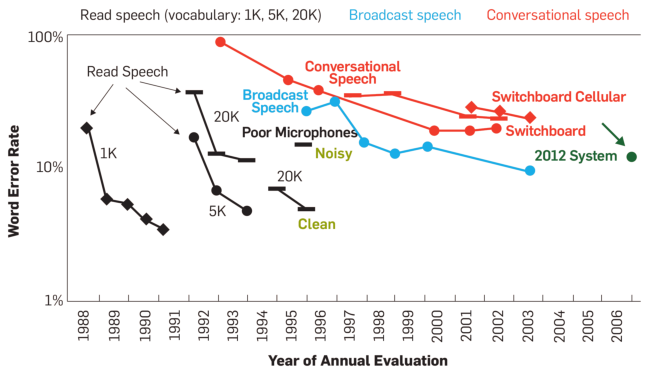
\includegraphics[width=.95\linewidth]{gfx/asr-performance-history.pdf}}
        \caption{Historical progress of speech recognition word error rate on more and more
difficult tasks [Huang et al. 2014].}
        \label{fig:asr-history}
\end{figure}

The results reported in \autoref{fig:asr-history} are often from papers from large IT companies, such as Google, Apple or Microsoft, which have at their disposal not only the best algorithms and computer power in the world, but also the largest databases, some of them with up to 2,000 hours for training \cite{Huang2014}. Nonetheless, \ac{ASR} is such a difficult task, that, despite having all set, the best results reported are still around 12\% for conversational speech  \cite{Huang2014}. This means that a short sentence with 4 words will be fully recognised only 60\% of the times. 

Such result for conversational speech is mainly due to the large amount of linguistic variability. Language varies not only among speakers (the so-called inter-speaker variability), but also within the same speaker (intra-speaker) \citep{Benzeghiba2007}.  Considering inter-speaker differences, factors such as gender, age, social, and regional 
origin, health and emotional state might have a huge impact on the speech signal \citep{Benzeghiba2007}.
Sociolinguistics has long known that gender affects language usage. In fact, men and women tend to use different language constructions.
In her seminal paper on gender sociolinguistics, \citet{Lakoff1973} found that, in women's speech, strong expressions 
of feeling are avoided, uncertainty is favoured, and means of expression in regard to subject-matter deemed ``trivial'' to the 
``real'' world are elaborated. 

Disregarding social aspects, men, women and children's speech are also contrasting due to morphological differences
in their vocal tract. Sex and development influence body size, and there is a strong correlation between vocal tract length and body size 
(either height or weight); in addition to this, the relative proportions of men and women's oral and pharyngeal cavity are unlike 
\cite{Fitch1999}. \autoref{fig:vocal-tract-morphology-sex} presents a comparison between height and
vocal tract length for men, women and children. \autoref{fig:vocal-tract-morphology} presents a model of the vocal tract morphology considering
age.

\begin{figure}[!ht]
        \noindent\makebox[\textwidth]
        {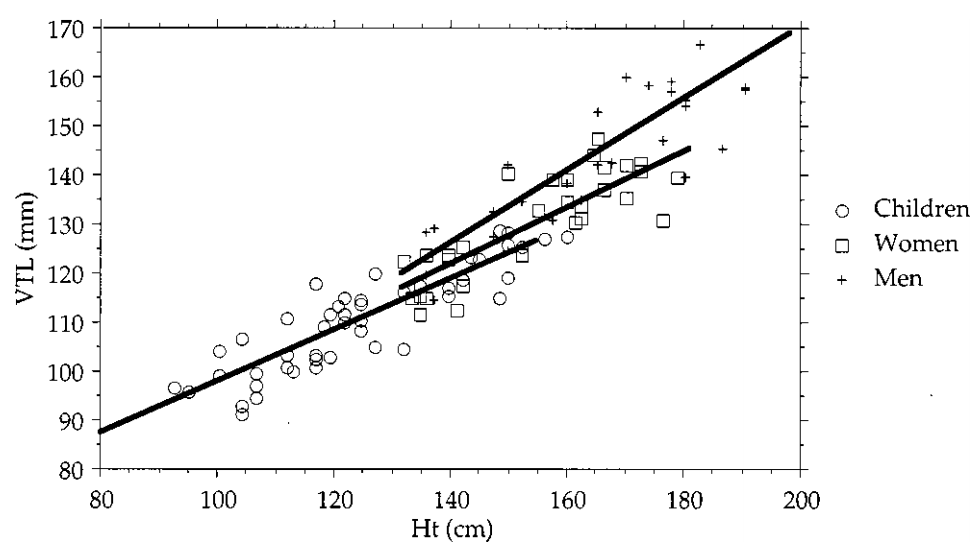
\includegraphics[width=.66\linewidth]{gfx/vocal-tract-size-sex.png}}
        \caption{Height (cm) versus vocal tract length (mm) [Fitch and Giedd 1999].}
        \label{fig:vocal-tract-morphology-sex}
\end{figure}

\begin{figure}[!ht]
        \noindent\makebox[\textwidth]
        {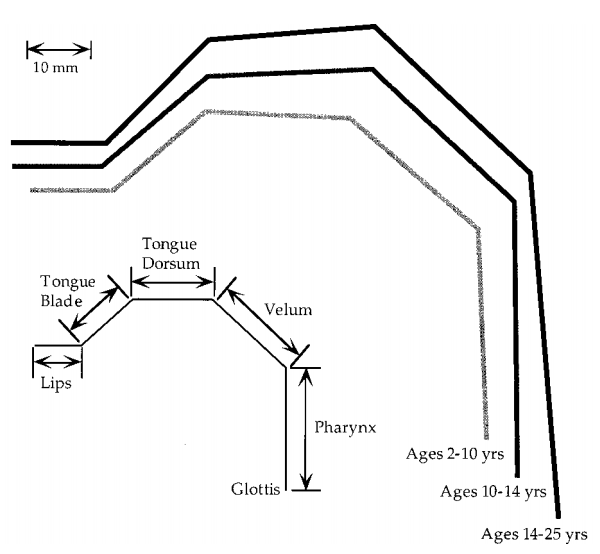
\includegraphics[width=.66\linewidth]{gfx/vocal-tract-size-gender.png}}
        \caption{Averaged vocal tract morphology [Fitch and Giedd 1999].}
        \label{fig:vocal-tract-morphology}
\end{figure}

As one can observe, men's vocal tract are longer than women's, followed by the children's. These differences 
affect the speech signal thoroughly, especially in what concerns to the \ac{F0}. \ac{F0} can be defined as the 
lowest frequency in the signal counting from zero. \autoref{fig:f0-age-sex} compares the \ac{F0} values
between male and females considering aging.

\begin{figure}[!ht]
        \noindent\makebox[\textwidth]
        {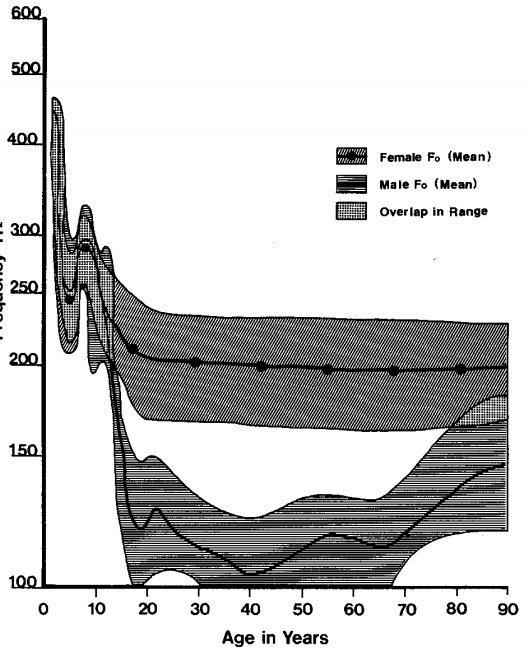
\includegraphics[width=.66\linewidth]{gfx/f0-age-sex.png}}
        \caption{F0 and pitch sigma versus age for males and females.}
        \label{fig:f0-age-sex}
\end{figure}

One can notice from \autoref{fig:f0-age-sex}, that no difference is found between male and female voice at a very young age. 
In fact, boys and girls have roughly the same \ac{F0} values. However, when they reach puberty, differences begin to appear. 
This period is commonly called the voice mutation or voice change, when the \ac{F0} for male voice undergoes a huge drop, whereas 
for female voice the drop is quite small. In terms of perception, this is the period when the male voice lowers and becomes deeper.

Back to \autoref{tab:comparison-human-mach}, it is interesting to notice that humans
performed better in all speech recognition tasks, but one: ``Clean speech based on trigram sentences''.
This very task consists of recognising sentences which were randomly generated using the WSJ trigram language model. 
Therefore, humans had no advantage over machines in what concerns to syntactic or semantic knowledge. 
This result highlights one of the most important aspects of human hearing, that is, that we humans make a large use of syntactic, 
semantic and also pragmatic information in order to understand speech. Hearing does not take into account 
the acoustic signal, but the whole context. Language is a social tool, which aims at successfull interaction. When someone is at a restaurant and says to a waiter
[\textipa{aIs"pli:z}], the waiter has no doubt that this sequence of phones refers to ``ice, please'' and not ``eyes, please'', albeit they sound exactly the same. Such sequences of phones might cause confusion at the phonetic level, but
in higher linguistic levels, such as pragmatics, their difference is quite clear. One simply does not order ``eyes'' to waiter.

One of the central problems in \ac{ASR} is how to deal with noisy audio data. It is long known that the performance of 
speech recognition systems greatly degrate when the environmental or the recording conditions are not controlled, 
thus allowing unwanted residual sounds to appear in the signal. In acoustics, any type of sound that is not the one
you are willing to analyse is considered noise. As a result from this, in speech recognition, the hiss of a fan, 
the buzz that a computer cooler makes, car horns on the street and so on are all regarded as noise. Even someone's voice
can be regarded as noise. Consider, for instance, that you are trying to recognise John's speech in an application, 
but Mary is close to him talking on the phone, to the extent that traces of her voice are added to the signal. In this
scenario, Mary's voice is actually noisy data, as it is undesirable for the given purpose. 

\subsection{The fundamental equation}

Roughly speaking the purpose of an \ac{ASR} system is to transform, in a precise and efficient way, the acoustic parameters of a speech signal into readable text \cite{Rabiner2007}.
Basically, all statistical methods of \ac{ASR} are dedicated into solving one fundamental 
equation, which can be described as follows. Let $O$ be a sequence of observable acoustic 
feature vectors and $W$ be a word sequence, the most likely word sequence $W*$ is given by:

\begin{equation}{\label{eq:fund-asr}}
W*= \arg\max_{W}P(W|O)
\end{equation}

To solve this equation straightforwadly, one would require a discriminative model,
capable of estimating the probability of $W$ directly from a set of observations $O$ \cite{Gales2008}.
However, \ac{HMM} are generative models and are not adequate for solving this equation and,
therefore, we apply Bayes' Theorem to Equation~\ref{eq:fund-asr}, ending up with:

\begin{equation}
W*= \arg\max_{W}\frac{P(O|W)P(W)}{P(O)}
\end{equation}

As one might notice, we can apply a generative model to calculate the conditional probability term of this
equation, that is, the probability of the observation sequence $O$ given a word sequence $W$, hence $P(O|W)$.
At first, it might seem counter-intuitive to conceive a generative model for data analysis, since the 
data is already available, i.e. $O$ is known before-hand. In order to understand how generative models are used for data analysis, a mental trick is necessary \cite{Fink2014}. First, one must assume that the data was generated through a process which obeys statistical regularities. Then, a model is trained over the observable data, in order to generate the data itself; in other words, the model is used to calculate the probability of generating the available data. Assuming that the observable data follows a regular pattern which represents the underlying hidden states, the models which are estimated can be said to encode the information of such hidden states. The estimated models are thus used to determine what the state sequence that generates a certain sequence of outputs with the highest probability is.

For a single audio input, which we want to decode, the audio is already fixed, so the 
probability of the observable acoustic feature vectors $P(O)$ is a constant and, therefore, 
might be discarded. Thus the final fundamental equation is simplified to:

\begin{equation}
W*= \arg\max_{W}P(O|W)P(W)
\end{equation}
$P(O|W)$, the probability of an observable acoustic feature vector given a word sequence, is calculated by 
an acoustic model. In turn, $P(W)$, the \emph{a priori} probability of words is reckoned by a language model.

\subsection{Architecture of an Automatic Speech Recognition}

\ac{ASR}s can be grouped into three categories that take into account the complexity of the task they perform: (i) isolated-word recognition; (ii) command and control systems, in other words, speech recognition systems which are able to recognise pre-defined sentences or expressions; and (iii) large vocabulary continuous speech recognition \cite{Rabiner1997}.

Isolated-word recognition are often used by call centers, in \ac{IVR}, with their well-known voice menus: ``For recent orders say 'order'; for technical support say 'support' (...)''. 

The second type of \ac{ASR} is more robust in comparison to the first, being able to recognise pre-defined commands or sentences, which are usually represented through grammars, such as a \ac{CFG}. An example of application of this type involves the use of voice commands in computers, mobile phones and hands-free systems in cars. In those systems, sentences such as ``turn on the radio'' or ``what is the closest Starbucks'' are said and the command is recognised. 

Large vocabulary continuous speech recognition comprises the most complex type of ASR, being capable of processing users' spontaneous speech.
Large vocabulary continuous speech recognition is present in a wide range of applications, such as voice search, personal assistants, dictation systems, domotic, Computer Assisted Pronunciation Training, etc. These systems usually have three modules: (i) a language model, (ii) an acoustic model and (iii) a pronunciation model or dictionary.

The language model is used to estimate the a priori probability of the sequence of the words. The pronunciation model, in its turn, plays the role of a bridge between the language and the acoustic models, as it possesses the words which comprise the lexicon of the recogniser and their corresponding phonetic forms. Finally, the acoustic model is used to calculate the likelihood of the observation. \autoref{fig:asr-gen-architecture} illustrates the basic architecture of an ASR system.

\begin{figure}[!ht]
        \noindent\makebox[\textwidth]
        {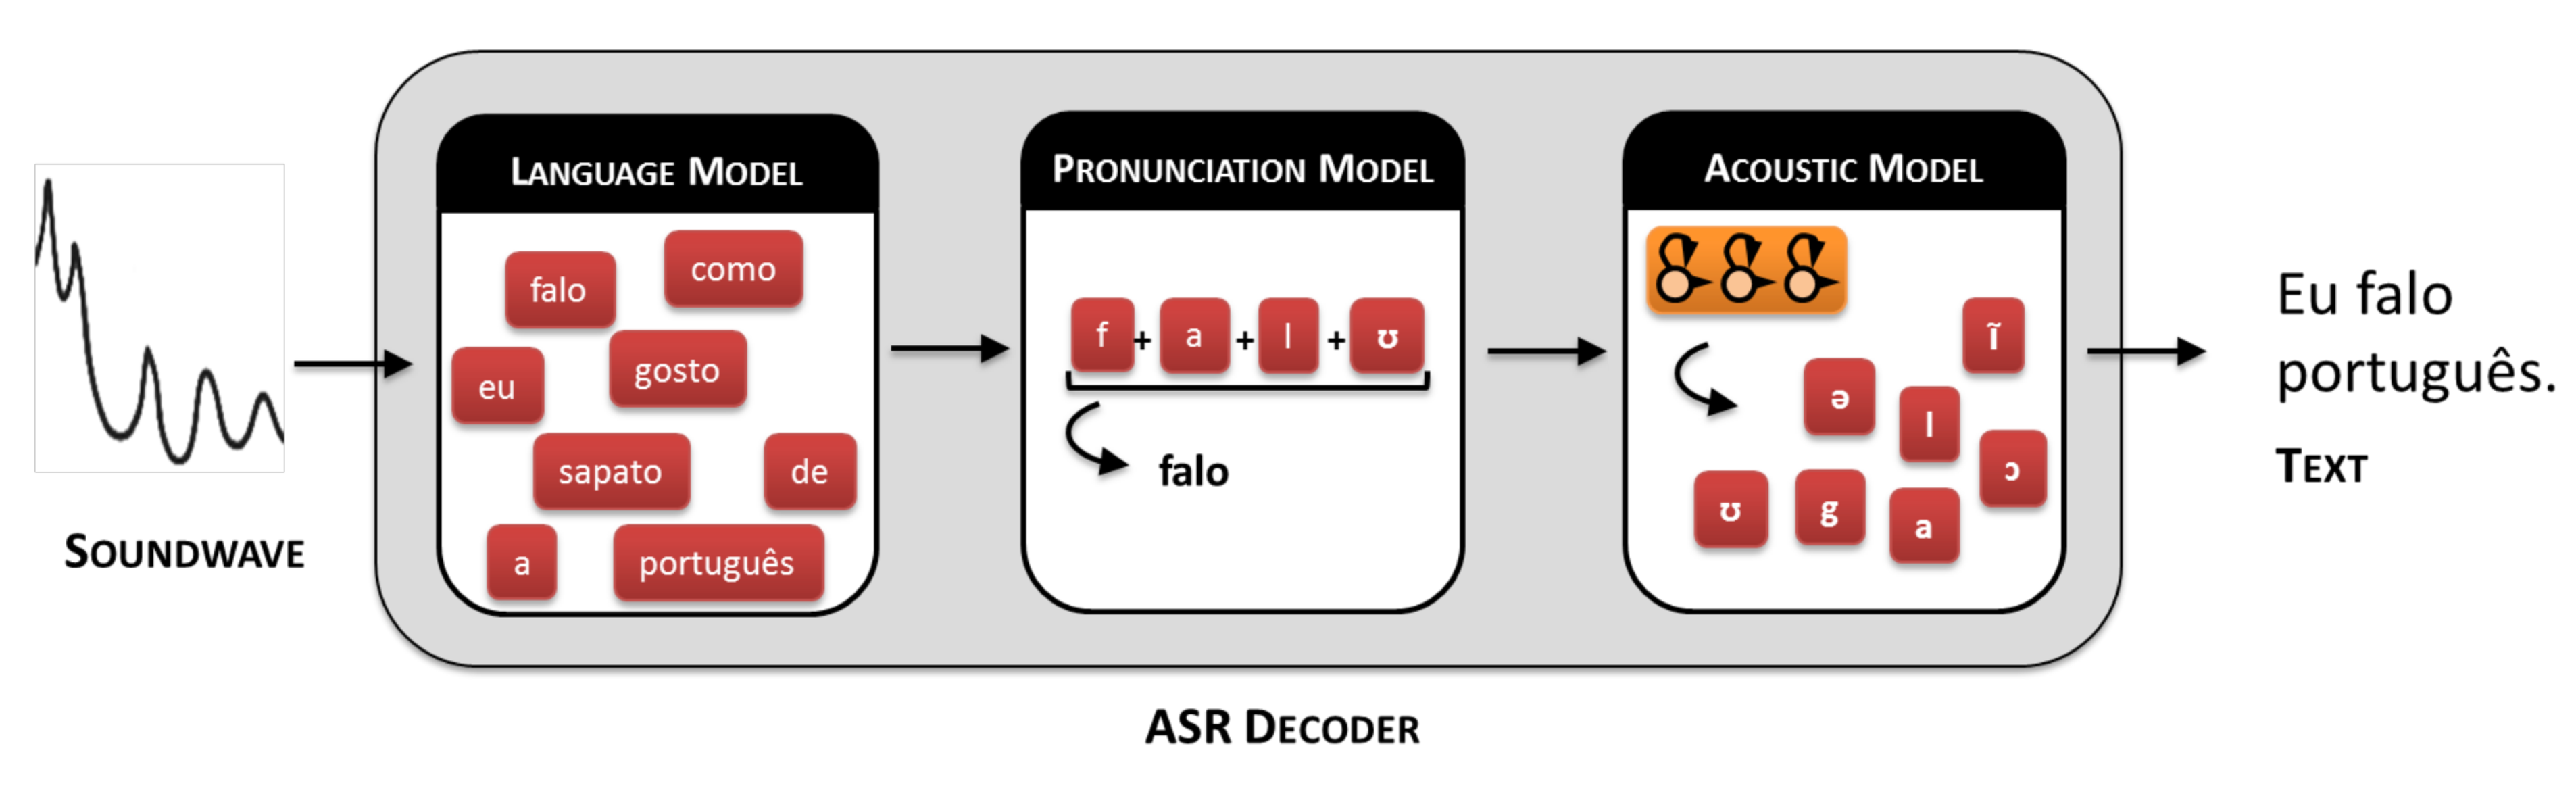
\includegraphics[width=.95\linewidth]{gfx/asr-architecture.pdf}}
        \caption{Architecture of a continuous speech recognition system.}
        \label{fig:asr-gen-architecture}
\end{figure}

The acoustic model processes the acoustic signal of the speech. This model does so in order for it to infer what sound segments comprise the speech, usually by means of using phones or triphones. In HMM-based recognisers, the task of processing the acoustc signal is carried out  estimating the most likely observed acoustic states as well as their transition probabilities. On the other hand, the pronunciation model provides us with the correspondence between phones and words sequences in the language. In the example, such model maps on the sequence of phones [\textipa{falU}] in the word "falo". The language model, in its turn, estimates the ordering of the most likely words in the language. 

\subsection{Hidden Markov Models in Speech Recognition}

\ac{HMM}s are the most widespread and succesful paradigm in \ac{ASR}. When \ac{HMM}s were first applied
to speech recognition in the late 70's, they were completely revolutionary.
Up until recently, \ac{HMM} had basically a monopoly in \ac{ASR}, being used in virtually all state-of-the-art systems. Since 2011, \ac{DNN} \cite{Povey2011} has gained a lot of popularity, seeming to be the next prominent paradigm in \ac{ASR}.
This is so due to \ac{HMM} having been applied
to \ac{ASR} since the late 70's, and having gathered the best results until recently.

An \ac{HMM} is a statistical Markov model in which the states are assumed to be hidden, i.e. they are
not directly visible, only the state's outputs are observable \cite{Fink2014}. Each state has a probability distribution over the possible output tokens, in such a way that the output generated by the HMM states provides some information about the hidden sequence of states which was traversed.  The simplest form of Markov models are Markov chain models, 
which represent a system with a set of spaces in which transitions from one state to another occur. 
Within Markov processes, systems are assumed to be memoryless, that is, the conditional probability
of future states is only dependent on the present state. To put it another way, Markov models assume that,
given a certain system with states and transitions, the current state does not depend upon the 
sequence of events that preceded it, the so-called Markov property. 

\citet{Kohlschein2006} \cite{Kohlschein2006} formally defines \ac{HMM}s as a 5-tuple $\lambda = \left (Q, O, \Pi, A, B\right )$, where $Q = \left \{q_1, q_2, q_3, ..., q_N\right \}$  is a set of $N$ states. $O = \left \{o_1, o_2, o_3, ..., o_T\right \}$ is a set of $T$ observations taken from time $t = 1$ to $t = T$. At each time $t$ it is assumed that the system will be at a specific state $q$, which is hidden; only the observations are directly visible. $\Pi = \left \{\pi_i \right \}$ is a vector with the initial state probabilities, in that
\begin{equation}
\pi_i = Pr(q_i), t = 0
\end{equation}
$A = [a_{ij}]$ is matrix with the state transition probabilities so that
\begin{equation}
a_{ij} = P(q_t = j | q_{t-1} = i),  1 \leq, i, j \leq N
\end{equation}
and $B = [b_{jt}]$ is a matrix with the emission probability of each state. Assuming a \ac{GMM} to model the state emission probabilities -- the so-called GMM/HMM model; we can define that, for a state $j$, the probability $b_j(o_t)$ of generating $o_t$ is given by
\begin{equation}
 b_j(o_t) = \prod_{s=1}^{S}\left [ \sum_{m=1}^{M_{js}} c_{jsm}\mathcal{N}(o_{st}; \mu_{jsm}, \Sigma_{jsm}) \right ]^{\gamma_s}
\end{equation}
where $\gamma s$ is a stream weight, with default value is one, $M_{js}$ is the number of mixture components in state $j$ for stream $s$, $c_{jsm}$ is the weight of the $m$\textsuperscript{th} component and $\mathcal{N}(\cdot; \mu_{jsm}, \Sigma_{jsm})$ is a multivariate Gaussian with mean vector $\mu$ and covariance matrix $\Sigma$, that is
\begin{equation}
 \mathcal{N}(o; \mu, \Sigma) = (\sqrt{(2\pi)^{n}\left |\Sigma\right |})^{-e^{-\frac{1}{2}(o-\mu)^{T}\Sigma^{-1}(o-\mu)}}
\end{equation}
where $n$ is the dimensionality of $o$.

The following constraints apply:
\begin{equation}
a_{ij} > 0
\end{equation}
that is, the probability of moving from any state $i$ to $j$ is not null, and
\begin{equation}
\sum_{j=1}^{N} a_{ij} = 1, \forall i
\end{equation}

\subsection{Feature Extraction}

Feature extraction is an important part of speech recognition systems. The feature extraction 
phase is responsible for identifying or enhancing the components of the signal that are relevant 
for recognising speech sounds, while discarding or diminishing the effect of unuseful information, 
such as background noise. With respect to speech parameterisation, \ac{MFCC} are definitely the
standard. \ac{MFCC} have been widely used in \ac{ASR} systems for almost three decades \cite{Davis1980}, and 
they are present on the many important speech recognition toolkits, such as \ac{HTK}, Sphinx, \ac{RASR} and Kaldi.
Before we go into further details about these features, it is noteworthy to provide some background information about speech recording and coding.

Speech is recorded by using a microphone -- nothing new so far.
Despite the many types of available microphones (condenser, capacitor, pyezoeletric, laser, etc.), their design
remain basically the same as the carbon microphone invented by David Hughes two centuries ago \cite{Robjohns2010}.
A microphone is simply an acoustic-to-electric sensor, which converts variations in air pressure (that is, sound)
into an electrical signal. Microphones have a very thin membrane, called diaphragm, which vibrates when struck by 
sound waves.  When the diaphragm vibrates, it puts to move a sensitive capsule attached to it, 
that converts its movement into electrical pulses. Most of the current microphones are based on electromagnetic induction (a.k.a dynamic microphones).

After capturing speech through a microphone, one usually wants to store it for later access. In order
to store speech digitally on a computer, a coding scheme is mandatory. In the literature, many coding schemes have
been proposed, such as linear PCM, $\mu$-law, A-law PCM, APCM, DPCM, DM, and ADPCM \cite{Huang2001}. The details of 
each type of speech coder is beyond the scope of this dissertation. 

For our purposes, Linear PCM is the only relevant one, since it is the standard way of storing audios in digital format. \ac{PCM} is a type of analogue-to-digital conversion, which constitutes the basis of the WAV digital audio format, together
with other lossless formats, such as AIF and AU
\footnote{Other types of popular audio files which use lossy data compression, such as MP3, WMA, OGG or AAC (a format common to 
DivX videos) do not use PCM.}. 
PCM coding is based on two properties: (i) a sampling rate of the audio and a (ii) bit depth. The sampling rate determines the
number of audio samples that are taken per second from the signal, in turn the bit depth is the number of bits 
bits adopted to represent each sample. Both values must be constant and should be defined prior to recording (actually coding) an audio. 
The sampling and the bit depth are closely related to the audio quality, that is, the higher the sampling and the depth
the better the fidelity of the digital audio to the analogue speech signal.

Linear PCM assumes that the discrete signal $x[n]$ is bounded, that is,
\begin{equation}
|x[n]| \leq X_{max} 
\end{equation}
and that the quantisation step $\Delta$ is uniform for all consecutive levels of $x[n]$
\begin{equation}
x[n] - x[n-1] = \Delta
\end{equation}

Assuming a binary code, the number of levels which can be represented by PCM is $N=2^B$, where $B$ is the bit depth, which indicates
the audio resolution. According to \citep{Huang2001}, speech could be represented in an intelligible way by using 7 bits. However, in 
practice, applications use values no lower than 11 bits to guarantee communication efficiency. For instance, CDs make use of 16-bit 
linear PCM, whereas DVD-Audio and Blu-Ray discs can support up to 24 bits.

Although linear PCM files are able to carry all the necessary auditory information -- after all, we are able to listen to them and
recognise the speech, the music or the noise recorded in them -- they are not useful for speech recognition purposes when used directly to feed the recognizer. This occurs 
because, from the phonological point of view, very little can be said based on the waveform itself \citep{Shrawankar2010}. Despite being composed by the same pure tones, complex waves can be completely distinct from one another in terms of their waveform, due to phase shifts, also known as phase offsets. In-phase and out-of-phase waves (\autoref{fig:in-phase-waves} and
\autoref{fig:out-of-phase-waves}) are represented differently, and this adds much variability to the waveform, in such a way that
the signal waveform becomes unsuitable for human analysis and consequently for being used as a raw input in \ac{ASR} systems. 

\begin{figure}[!ht]
        \noindent\makebox[\textwidth]
        {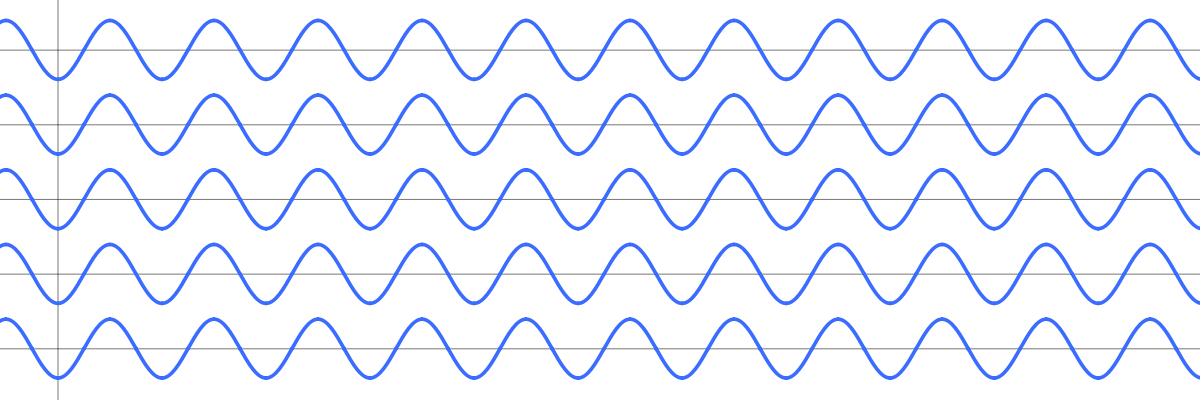
\includegraphics[width=.66\linewidth]{gfx/in-phase-waves.png}}
        \caption{Example of in-phase waves.}
        \label{fig:in-phase-waves}
\end{figure}

\begin{figure}[!ht]
        \noindent\makebox[\textwidth]
        {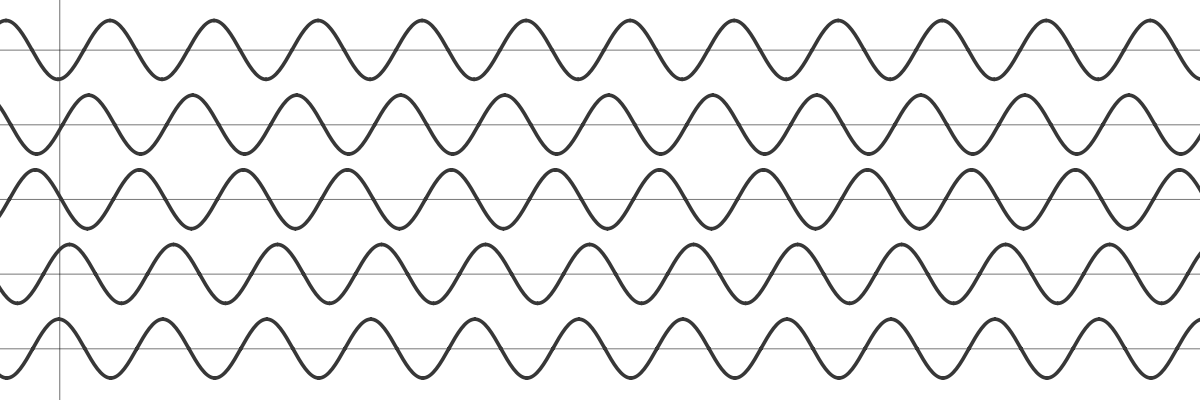
\includegraphics[width=.66\linewidth]{gfx/out-of-phase-waves.png}}
        \caption{Example of out-of-phase waves.}
        \label{fig:out-of-phase-waves}
\end{figure}

Another way of representing the audio information, which is more meaningful for human reading
or computer analysis is, through short-term spectrum. Short-term spectra are obtained by applying
a Discrete Time Fourier transform to a windowed signal. At first, the signal is divided
into uniformly-spaced periods with a sliding window. For speech recognition, the window size is usually defined as 25 ms, 
with a frame shift of 10 ms, the audio information is extracted every 10 ms with 15 ms of overlapping
among adjacent frames \cite{Huang2001}. \autoref{fig:audio-windowing} contains an example of a windowing process (in this case, 
with 50\% overlapping).

\begin{figure}[!ht]
        \noindent\makebox[\textwidth]
        {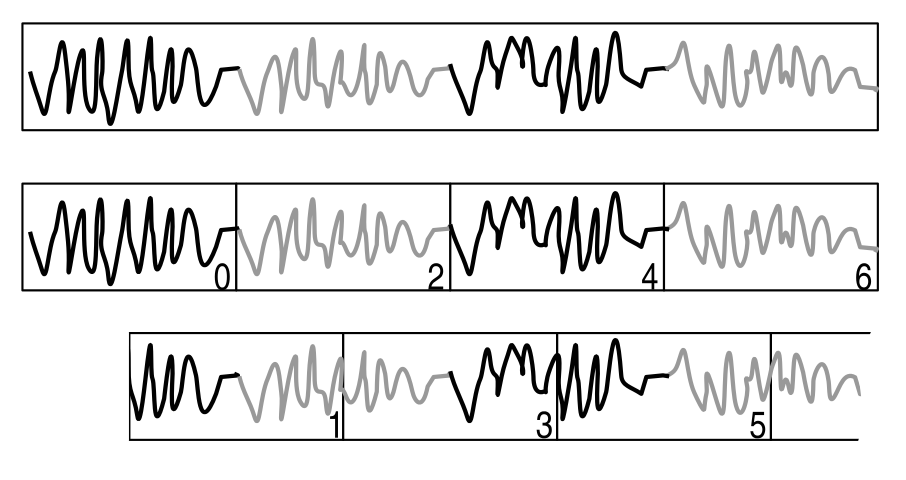
\includegraphics[width=.66\linewidth]{gfx/audio-windowing.png}}
        \caption{Illustration of an original audio recording (the upper waveform) divided into two
offset sequences of analysis windows (two lower waveforms) with 50\% overlapping frames [McLoughlin 2009].}
        \label{fig:audio-windowing}
\end{figure}

These windows values are based on two assumptions: (i) that within 25 ms the signal is stationary, i.e.
the phonatory system is not moving; (ii) that at least a period of each relevant speech frequency will 
be within this window.

After windowing the signal a Fourier transform is applied into each window so as to obtain
a series of frequency spectra, i.e. a series of representation of the signal in the frequency domain instead of the time domain. As it can be noticed in \autoref{fig:audio-windowing}, as the frame shift is smaller than the window size, the windowing process extracts many redundant information. 

Such transform is based on the Fourier theorem, which states that any periodic waveform can be approximated as closely as desired as the sum of a series of pure sine waves. In other words, when the signal is not periodic,  the Fourier transform is able to analyse a short-term of the signal, containing a complex wave, and to output what the amplitude of the pure tones which form this complex wave is.

Feature extraction must then be performed in stored audio files in order to extract relevant information from the waveform and discard redundant or unwanted signal characteristics. As already mentioned before, the two most traditional techniques for speech feature extraction, over the past decades, have been the \ac{MFCC} \cite{Davis1980} and the \ac{PLP} \cite{Hermansky1990}. Both parameterisation methods are based on the short-term spectrum of speech. For speech recognition purposes, \ac{MFCC} features usually show better performance when compared to \ac{PLP}. For this reason, in this thesis we are only going to present \ac{MFCC} features \cite{Mporas2007}.

\subsection{MFCC Features}

\ac{MFCC} is a type of speech parameterisation is the result of a cosine transform of the logarithm of the short-term energy spectrum expressed over a mel scale \cite{Davis1980}. \ac{MFCC} features tries to reduce the feature dimensionality of a sound Fourier spectrum, by applying some concepts of Psychoacoustics and Psychophysics in order to the extract a vector with relevant values from the spectrum. The aim is to represent speech data in a compressed format, by eliminating information which are not pertinent to the phonetic analysis and to enhance the aspects of the signal which contribute to the detection of phonetic differences \cite{Davis1980}.

From Psychoacoustics, \ac{MFCC}s use the notion that humans do not perceive frequency through a linear scale, but through a scale which seems to be linear-spaced in frequencies below 1000 Hz and logarithmic in frequecies above 1000 Hz\footnote{This is not entirely true. As shown by \citet{Umesh1999}, in fact, there are no two distinguishable regions in terms of statistical significance. But the idea that we perceive low frequencies better than high ones still prevails.}, the so-called mel scale (named after \emph{mel}ody). The scale is based on experiments with simple tones in which individuals are required to separate frequency values into four equal intervals or to adjust the frequency of a stimulus to be half as high as another reference tone \cite{Huang2001}. The reference point between a mel scale and a linear frequency scale is 1000 mels, which corresponds to a 1000 Hz tone, 40 dB above the absolute threshold of hearing. Since it was first introduced by \citet{Stevens1937}, the scale has been revisited many times \cite{Umesh1999}, but a common formulation, according to \citet{Huang2001} is:
\begin{equation}
 M(f) = 1125 ln(1 + f / 700)
\end{equation}
where $f$ is the input frequency in Hz. For better visualization, the scale is plotted in \autoref{fig:mel-scale}.

\begin{figure}[!ht]
        \noindent\makebox[\textwidth]
        {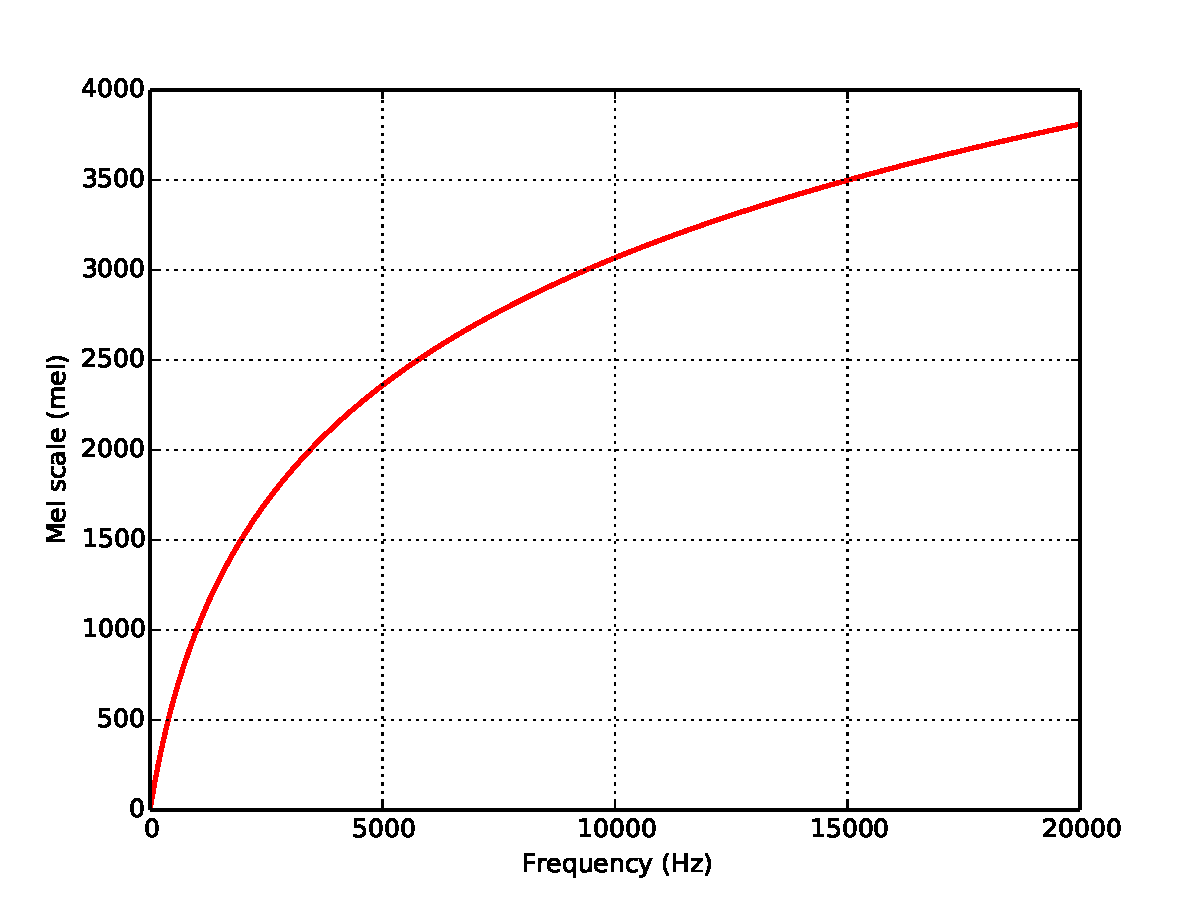
\includegraphics[width=0.7\paperwidth]{gfx/mel-scale.pdf}}
        \caption{Mel scale versus a linear frequency scale.}\label{fig:mel-scale}
\end{figure}

%*****************************************
%*****************************************
%*****************************************
%*****************************************
%*****************************************